\documentclass[twoside]{book}

% Packages required by doxygen
\usepackage{fixltx2e}
\usepackage{calc}
\usepackage{doxygen}
\usepackage[export]{adjustbox} % also loads graphicx
\usepackage{graphicx}
\usepackage[utf8]{inputenc}
\usepackage{makeidx}
\usepackage{multicol}
\usepackage{multirow}
\PassOptionsToPackage{warn}{textcomp}
\usepackage{textcomp}
\usepackage[nointegrals]{wasysym}
\usepackage[table]{xcolor}

% Font selection
\usepackage[T1]{fontenc}
\usepackage[scaled=.90]{helvet}
\usepackage{courier}
\usepackage{amssymb}
\usepackage{sectsty}
\renewcommand{\familydefault}{\sfdefault}
\allsectionsfont{%
  \fontseries{bc}\selectfont%
  \color{darkgray}%
}
\renewcommand{\DoxyLabelFont}{%
  \fontseries{bc}\selectfont%
  \color{darkgray}%
}
\newcommand{\+}{\discretionary{\mbox{\scriptsize$\hookleftarrow$}}{}{}}

% Page & text layout
\usepackage{geometry}
\geometry{%
  a4paper,%
  top=2.5cm,%
  bottom=2.5cm,%
  left=2.5cm,%
  right=2.5cm%
}
\tolerance=750
\hfuzz=15pt
\hbadness=750
\setlength{\emergencystretch}{15pt}
\setlength{\parindent}{0cm}
\setlength{\parskip}{3ex plus 2ex minus 2ex}
\makeatletter
\renewcommand{\paragraph}{%
  \@startsection{paragraph}{4}{0ex}{-1.0ex}{1.0ex}{%
    \normalfont\normalsize\bfseries\SS@parafont%
  }%
}
\renewcommand{\subparagraph}{%
  \@startsection{subparagraph}{5}{0ex}{-1.0ex}{1.0ex}{%
    \normalfont\normalsize\bfseries\SS@subparafont%
  }%
}
\makeatother

% Headers & footers
\usepackage{fancyhdr}
\pagestyle{fancyplain}
\fancyhead[LE]{\fancyplain{}{\bfseries\thepage}}
\fancyhead[CE]{\fancyplain{}{}}
\fancyhead[RE]{\fancyplain{}{\bfseries\leftmark}}
\fancyhead[LO]{\fancyplain{}{\bfseries\rightmark}}
\fancyhead[CO]{\fancyplain{}{}}
\fancyhead[RO]{\fancyplain{}{\bfseries\thepage}}
\fancyfoot[LE]{\fancyplain{}{}}
\fancyfoot[CE]{\fancyplain{}{}}
\fancyfoot[RE]{\fancyplain{}{\bfseries\scriptsize Generated by Doxygen }}
\fancyfoot[LO]{\fancyplain{}{\bfseries\scriptsize Generated by Doxygen }}
\fancyfoot[CO]{\fancyplain{}{}}
\fancyfoot[RO]{\fancyplain{}{}}
\renewcommand{\footrulewidth}{0.4pt}
\renewcommand{\chaptermark}[1]{%
  \markboth{#1}{}%
}
\renewcommand{\sectionmark}[1]{%
  \markright{\thesection\ #1}%
}

% Indices & bibliography
\usepackage{natbib}
\usepackage[titles]{tocloft}
\setcounter{tocdepth}{3}
\setcounter{secnumdepth}{5}
\makeindex

% Hyperlinks (required, but should be loaded last)
\usepackage{ifpdf}
\ifpdf
  \usepackage[pdftex,pagebackref=true]{hyperref}
\else
  \usepackage[ps2pdf,pagebackref=true]{hyperref}
\fi
\hypersetup{%
  colorlinks=true,%
  linkcolor=blue,%
  citecolor=blue,%
  unicode%
}

% Custom commands
\newcommand{\clearemptydoublepage}{%
  \newpage{\pagestyle{empty}\cleardoublepage}%
}

\usepackage{caption}
\captionsetup{labelsep=space,justification=centering,font={bf},singlelinecheck=off,skip=4pt,position=top}

%===== C O N T E N T S =====

\begin{document}

% Titlepage & ToC
\hypersetup{pageanchor=false,
             bookmarksnumbered=true,
             pdfencoding=unicode
            }
\pagenumbering{alph}
\begin{titlepage}
\vspace*{7cm}
\begin{center}%
{\Large Mavad }\\
\vspace*{1cm}
{\large Generated by Doxygen 1.8.13}\\
\end{center}
\end{titlepage}
\clearemptydoublepage
\pagenumbering{roman}
\tableofcontents
\clearemptydoublepage
\pagenumbering{arabic}
\hypersetup{pageanchor=true}

%--- Begin generated contents ---
\chapter{Class Index}
\section{Class List}
Here are the classes, structs, unions and interfaces with brief descriptions\+:\begin{DoxyCompactList}
\item\contentsline{section}{\hyperlink{structrnl_1_1DroneSoc}{rnl\+::\+Drone\+Soc} \\*Drone Socket common for planning and communication }{\pageref{structrnl_1_1DroneSoc}}{}
\item\contentsline{section}{\hyperlink{classrnl_1_1Interface}{rnl\+::\+Interface} }{\pageref{classrnl_1_1Interface}}{}
\item\contentsline{section}{\hyperlink{structrnl_1_1Nbt}{rnl\+::\+Nbt} \\*For parsing and serializing data of neighbouring nodes }{\pageref{structrnl_1_1Nbt}}{}
\item\contentsline{section}{\hyperlink{classrnl_1_1Planner}{rnl\+::\+Planner} \\*\hyperlink{classrnl_1_1Planner}{Planner} class. Flow ~\newline
}{\pageref{classrnl_1_1Planner}}{}
\item\contentsline{section}{\hyperlink{classrnl_1_1Properties}{rnl\+::\+Properties} }{\pageref{classrnl_1_1Properties}}{}
\item\contentsline{section}{\hyperlink{structrnl_1_1URMsg}{rnl\+::\+U\+R\+Msg} \\*This Structure Will be parsed as a Unicast Message. The ~\newline
communication will have this format. Each drone receives ~\newline
Unicast Message in this format. The parser will convert ~\newline
the received message into struct members. ~\newline
}{\pageref{structrnl_1_1URMsg}}{}
\item\contentsline{section}{\hyperlink{structrnl_1_1USMsg}{rnl\+::\+U\+S\+Msg} \\*This Structure Will be Serialized and sent as Unicast Message. The ~\newline
communication will have this format. Each drone sends ~\newline
Unicast Message in this format. The serializer will make a ~\newline
delimiter seperated string which will be passed onto the sockets ~\newline
for transmission. ~\newline
}{\pageref{structrnl_1_1USMsg}}{}
\end{DoxyCompactList}

\chapter{File Index}
\section{File List}
Here is a list of all documented files with brief descriptions\+:\begin{DoxyCompactList}
\item\contentsline{section}{include/\hyperlink{planner__config_8h}{planner\+\_\+config.\+h} \\*Configuration file for setting the serializing \& parsing of ns3 data to other formats. Contains the datatype for data encoding \& decoding and other static data variables }{\pageref{planner__config_8h}}{}
\item\contentsline{section}{include/\hyperlink{planner__ns3_8h}{planner\+\_\+ns3.\+h} \\*Planner class for the project }{\pageref{planner__ns3_8h}}{}
\item\contentsline{section}{include/\hyperlink{planner__ns3__utils_8h}{planner\+\_\+ns3\+\_\+utils.\+h} \\*Utility functions for Swarm Planner }{\pageref{planner__ns3__utils_8h}}{}
\item\contentsline{section}{include/{\bfseries ros\+\_\+linker.\+h} }{\pageref{ros__linker_8h}}{}
\item\contentsline{section}{src/\hyperlink{mavad__main_8cc}{mavad\+\_\+main.\+cc} \\*Exucatable file for simulation, contains the main function }{\pageref{mavad__main_8cc}}{}
\end{DoxyCompactList}

\chapter{Class Documentation}
\hypertarget{structrnl_1_1DroneSoc}{}\section{rnl\+:\+:Drone\+Soc Struct Reference}
\label{structrnl_1_1DroneSoc}\index{rnl\+::\+Drone\+Soc@{rnl\+::\+Drone\+Soc}}


Drone Socket common for planning and communication.  




{\ttfamily \#include $<$planner\+\_\+ns3.\+h$>$}



Collaboration diagram for rnl\+:\+:Drone\+Soc\+:\nopagebreak
\begin{figure}[H]
\begin{center}
\leavevmode
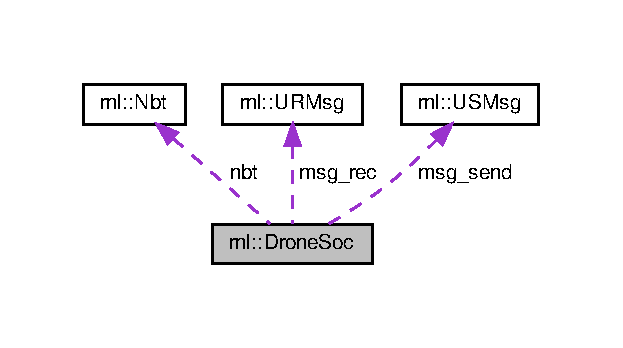
\includegraphics[width=299pt]{structrnl_1_1DroneSoc__coll__graph}
\end{center}
\end{figure}
\subsection*{Public Member Functions}
\begin{DoxyCompactItemize}
\item 
\mbox{\Hypertarget{structrnl_1_1DroneSoc_a064d6dcee6a438e84bc75a211757518a}\label{structrnl_1_1DroneSoc_a064d6dcee6a438e84bc75a211757518a}} 
\hyperlink{structrnl_1_1DroneSoc_a064d6dcee6a438e84bc75a211757518a}{Drone\+Soc} ()
\begin{DoxyCompactList}\small\item\em Construct a new Drone Soc object. \end{DoxyCompactList}\item 
void \hyperlink{structrnl_1_1DroneSoc_a21ec1cbe2adaefffc5f4472a59b07d6f}{send\+Packet} (ns3\+::\+Time pkt\+Interval, int n)
\begin{DoxyCompactList}\small\item\em send Packet after every pkt\+Interval. ~\newline
 This registers a callback which is periodically called \end{DoxyCompactList}\item 
void \hyperlink{structrnl_1_1DroneSoc_ab6c91121d046bf9632c1353c30ffde73}{send\+Bc\+Packet} (ns3\+::\+Time pkt\+Interval, int n)
\begin{DoxyCompactList}\small\item\em Send a broadcast packet. \end{DoxyCompactList}\item 
void \hyperlink{structrnl_1_1DroneSoc_a4945013e829ed896e2ca82699e62e711}{receive\+Packet} (ns3\+::\+Ptr$<$ ns3\+::\+Socket $>$ soc)
\begin{DoxyCompactList}\small\item\em Socket receiving callback. ~\newline
This function will be called as an interrupt if something is received at the socket end. \end{DoxyCompactList}\item 
\mbox{\Hypertarget{structrnl_1_1DroneSoc_a89739bd5df166ca8b53e56eb3b10ec77}\label{structrnl_1_1DroneSoc_a89739bd5df166ca8b53e56eb3b10ec77}} 
void \hyperlink{structrnl_1_1DroneSoc_a89739bd5df166ca8b53e56eb3b10ec77}{close\+Sender} ()
\begin{DoxyCompactList}\small\item\em Terminate all sockets and send shut down command for this nodea. \end{DoxyCompactList}\item 
\mbox{\Hypertarget{structrnl_1_1DroneSoc_a552f5f4e560c562ac249ff8f255f48c9}\label{structrnl_1_1DroneSoc_a552f5f4e560c562ac249ff8f255f48c9}} 
void \hyperlink{structrnl_1_1DroneSoc_a552f5f4e560c562ac249ff8f255f48c9}{update\+Send\+Msg} ()
\begin{DoxyCompactList}\small\item\em update send message with the correct parent location and parent id to follow \end{DoxyCompactList}\item 
void \hyperlink{structrnl_1_1DroneSoc_ace69ee9fbd96e334a32fb5d499c70588}{set\+Bc\+Sender} (ns3\+::\+Ptr$<$ ns3\+::\+Node $>$ node, ns3\+::\+Type\+Id tid)
\begin{DoxyCompactList}\small\item\em Setup the node for broadcasting. \end{DoxyCompactList}\item 
void \hyperlink{structrnl_1_1DroneSoc_a79565f4fa767a87e45e400e1ab0b03f8}{set\+Sender} (ns3\+::\+Ptr$<$ ns3\+::\+Node $>$ node, ns3\+::\+Type\+Id tid, const std\+::string \&ip)
\begin{DoxyCompactList}\small\item\em Initialize the sender. \end{DoxyCompactList}\item 
\mbox{\Hypertarget{structrnl_1_1DroneSoc_a7d39b630d3ace733b06e89879edacbbc}\label{structrnl_1_1DroneSoc_a7d39b630d3ace733b06e89879edacbbc}} 
void {\bfseries set\+Recv} (ns3\+::\+Ptr$<$ ns3\+::\+Node $>$ node, ns3\+::\+Type\+Id tid)
\item 
\mbox{\Hypertarget{structrnl_1_1DroneSoc_a7db06059f42f449bcf5b93aa299924dd}\label{structrnl_1_1DroneSoc_a7db06059f42f449bcf5b93aa299924dd}} 
void \hyperlink{structrnl_1_1DroneSoc_a7db06059f42f449bcf5b93aa299924dd}{set\+Req\+Drone} ()
\begin{DoxyCompactList}\small\item\em Set if more drone required at the boundary. \end{DoxyCompactList}\end{DoxyCompactItemize}
\subsection*{Public Attributes}
\begin{DoxyCompactItemize}
\item 
ns3\+::\+Ptr$<$ ns3\+::\+Socket $>$ \hyperlink{structrnl_1_1DroneSoc_a1d4ae61d59f86c1efe46ca221711f07e}{source}
\item 
ns3\+::\+Ptr$<$ ns3\+::\+Socket $>$ \hyperlink{structrnl_1_1DroneSoc_aedfa903020617a408194c3a1b2bf8f22}{source\+\_\+bc}
\item 
ns3\+::\+Ptr$<$ ns3\+::\+Socket $>$ \hyperlink{structrnl_1_1DroneSoc_ab7620aceca921deff3b7e929bcf539a9}{recv\+\_\+sink}
\item 
int \hyperlink{structrnl_1_1DroneSoc_a1e6c71ed4e33fedcf54e7d1dd28657df}{id}
\item 
int \hyperlink{structrnl_1_1DroneSoc_a4d79451257929fcbaa69092b40af3077}{anch\+\_\+id}
\item 
\mbox{\Hypertarget{structrnl_1_1DroneSoc_a3c7d1e51b1e69f01ad7835aaeea11178}\label{structrnl_1_1DroneSoc_a3c7d1e51b1e69f01ad7835aaeea11178}} 
int {\bfseries circle\+\_\+dir}
\item 
ns3\+::\+Vector3D \hyperlink{structrnl_1_1DroneSoc_a53076839aa6e66664611d82d848d864b}{anch\+\_\+pos}
\item 
\hyperlink{structrnl_1_1USMsg}{rnl\+::\+U\+S\+Msg} \hyperlink{structrnl_1_1DroneSoc_afc38c88754777ceef7195a4eacb870b9}{msg\+\_\+send}
\item 
\hyperlink{structrnl_1_1URMsg}{rnl\+::\+U\+R\+Msg} \hyperlink{structrnl_1_1DroneSoc_abc05fd0c4b80eb3bb6561c6b3d030797}{msg\+\_\+rec}
\item 
\hyperlink{structrnl_1_1Nbt}{rnl\+::\+Nbt} \hyperlink{structrnl_1_1DroneSoc_ae8065f9f2549546f32f8afdd4417dc58}{nbt}
\item 
std\+::vector$<$ ns3\+::\+Vector3D $>$ \hyperlink{structrnl_1_1DroneSoc_af6f5003ab01dd213cfed46f595e68694}{wpts}
\item 
ns3\+::\+Vector3D \hyperlink{structrnl_1_1DroneSoc_acd4150016d89ea9846c2c735c75470a0}{pos}
\item 
int \hyperlink{structrnl_1_1DroneSoc_a83abdfd1bc5cedf1a4effe48918a49a2}{lookaheadindex}
\item 
int \hyperlink{structrnl_1_1DroneSoc_a0551bc4498f75645a7a0fed0c3d2fb00}{toggle\+\_\+bc}
\end{DoxyCompactItemize}


\subsection{Detailed Description}
Drone Socket common for planning and communication. 

\subsection{Member Function Documentation}
\mbox{\Hypertarget{structrnl_1_1DroneSoc_a4945013e829ed896e2ca82699e62e711}\label{structrnl_1_1DroneSoc_a4945013e829ed896e2ca82699e62e711}} 
\index{rnl\+::\+Drone\+Soc@{rnl\+::\+Drone\+Soc}!receive\+Packet@{receive\+Packet}}
\index{receive\+Packet@{receive\+Packet}!rnl\+::\+Drone\+Soc@{rnl\+::\+Drone\+Soc}}
\subsubsection{\texorpdfstring{receive\+Packet()}{receivePacket()}}
{\footnotesize\ttfamily void rnl\+::\+Drone\+Soc\+::receive\+Packet (\begin{DoxyParamCaption}\item[{ns3\+::\+Ptr$<$ ns3\+::\+Socket $>$}]{soc }\end{DoxyParamCaption})}



Socket receiving callback. ~\newline
This function will be called as an interrupt if something is received at the socket end. 


\begin{DoxyParams}{Parameters}
{\em soc} & Socket at which the message will be received \\
\hline
\end{DoxyParams}
\mbox{\Hypertarget{structrnl_1_1DroneSoc_ab6c91121d046bf9632c1353c30ffde73}\label{structrnl_1_1DroneSoc_ab6c91121d046bf9632c1353c30ffde73}} 
\index{rnl\+::\+Drone\+Soc@{rnl\+::\+Drone\+Soc}!send\+Bc\+Packet@{send\+Bc\+Packet}}
\index{send\+Bc\+Packet@{send\+Bc\+Packet}!rnl\+::\+Drone\+Soc@{rnl\+::\+Drone\+Soc}}
\subsubsection{\texorpdfstring{send\+Bc\+Packet()}{sendBcPacket()}}
{\footnotesize\ttfamily void rnl\+::\+Drone\+Soc\+::send\+Bc\+Packet (\begin{DoxyParamCaption}\item[{ns3\+::\+Time}]{pkt\+Interval,  }\item[{int}]{n }\end{DoxyParamCaption})}



Send a broadcast packet. 


\begin{DoxyParams}{Parameters}
{\em pkt\+Interval} & Packet interval at which this needs to be called. ~\newline
The packet will be called after n $\ast$ pkt\+Interval\\
\hline
{\em n} & number of nodes in the swarm \\
\hline
\end{DoxyParams}
\mbox{\Hypertarget{structrnl_1_1DroneSoc_a21ec1cbe2adaefffc5f4472a59b07d6f}\label{structrnl_1_1DroneSoc_a21ec1cbe2adaefffc5f4472a59b07d6f}} 
\index{rnl\+::\+Drone\+Soc@{rnl\+::\+Drone\+Soc}!send\+Packet@{send\+Packet}}
\index{send\+Packet@{send\+Packet}!rnl\+::\+Drone\+Soc@{rnl\+::\+Drone\+Soc}}
\subsubsection{\texorpdfstring{send\+Packet()}{sendPacket()}}
{\footnotesize\ttfamily void rnl\+::\+Drone\+Soc\+::send\+Packet (\begin{DoxyParamCaption}\item[{ns3\+::\+Time}]{pkt\+Interval,  }\item[{int}]{n }\end{DoxyParamCaption})}



send Packet after every pkt\+Interval. ~\newline
 This registers a callback which is periodically called 


\begin{DoxyParams}{Parameters}
{\em pkt\+Interval} & Packet interval at which this needs to be called. ~\newline
The packet will be called after n $\ast$ pkt\+Interval\\
\hline
{\em n} & number of nodes in the swarm \\
\hline
\end{DoxyParams}
\mbox{\Hypertarget{structrnl_1_1DroneSoc_ace69ee9fbd96e334a32fb5d499c70588}\label{structrnl_1_1DroneSoc_ace69ee9fbd96e334a32fb5d499c70588}} 
\index{rnl\+::\+Drone\+Soc@{rnl\+::\+Drone\+Soc}!set\+Bc\+Sender@{set\+Bc\+Sender}}
\index{set\+Bc\+Sender@{set\+Bc\+Sender}!rnl\+::\+Drone\+Soc@{rnl\+::\+Drone\+Soc}}
\subsubsection{\texorpdfstring{set\+Bc\+Sender()}{setBcSender()}}
{\footnotesize\ttfamily void rnl\+::\+Drone\+Soc\+::set\+Bc\+Sender (\begin{DoxyParamCaption}\item[{ns3\+::\+Ptr$<$ ns3\+::\+Node $>$}]{node,  }\item[{ns3\+::\+Type\+Id}]{tid }\end{DoxyParamCaption})}



Setup the node for broadcasting. 


\begin{DoxyParams}{Parameters}
{\em node} & Node to setup broadcasting for \\
\hline
{\em tid} & Type id \\
\hline
\end{DoxyParams}
\mbox{\Hypertarget{structrnl_1_1DroneSoc_a79565f4fa767a87e45e400e1ab0b03f8}\label{structrnl_1_1DroneSoc_a79565f4fa767a87e45e400e1ab0b03f8}} 
\index{rnl\+::\+Drone\+Soc@{rnl\+::\+Drone\+Soc}!set\+Sender@{set\+Sender}}
\index{set\+Sender@{set\+Sender}!rnl\+::\+Drone\+Soc@{rnl\+::\+Drone\+Soc}}
\subsubsection{\texorpdfstring{set\+Sender()}{setSender()}}
{\footnotesize\ttfamily void rnl\+::\+Drone\+Soc\+::set\+Sender (\begin{DoxyParamCaption}\item[{ns3\+::\+Ptr$<$ ns3\+::\+Node $>$}]{node,  }\item[{ns3\+::\+Type\+Id}]{tid,  }\item[{const std\+::string \&}]{ip }\end{DoxyParamCaption})}



Initialize the sender. 


\begin{DoxyParams}{Parameters}
{\em node} & node \\
\hline
{\em tid} & type id \\
\hline
{\em ip} & IP of the sending socket \\
\hline
\end{DoxyParams}


\subsection{Member Data Documentation}
\mbox{\Hypertarget{structrnl_1_1DroneSoc_a4d79451257929fcbaa69092b40af3077}\label{structrnl_1_1DroneSoc_a4d79451257929fcbaa69092b40af3077}} 
\index{rnl\+::\+Drone\+Soc@{rnl\+::\+Drone\+Soc}!anch\+\_\+id@{anch\+\_\+id}}
\index{anch\+\_\+id@{anch\+\_\+id}!rnl\+::\+Drone\+Soc@{rnl\+::\+Drone\+Soc}}
\subsubsection{\texorpdfstring{anch\+\_\+id}{anch\_id}}
{\footnotesize\ttfamily int rnl\+::\+Drone\+Soc\+::anch\+\_\+id}

Anchoring Id if any \mbox{\Hypertarget{structrnl_1_1DroneSoc_a53076839aa6e66664611d82d848d864b}\label{structrnl_1_1DroneSoc_a53076839aa6e66664611d82d848d864b}} 
\index{rnl\+::\+Drone\+Soc@{rnl\+::\+Drone\+Soc}!anch\+\_\+pos@{anch\+\_\+pos}}
\index{anch\+\_\+pos@{anch\+\_\+pos}!rnl\+::\+Drone\+Soc@{rnl\+::\+Drone\+Soc}}
\subsubsection{\texorpdfstring{anch\+\_\+pos}{anch\_pos}}
{\footnotesize\ttfamily ns3\+::\+Vector3D rnl\+::\+Drone\+Soc\+::anch\+\_\+pos}

Circling direction Anchoring position \mbox{\Hypertarget{structrnl_1_1DroneSoc_a1e6c71ed4e33fedcf54e7d1dd28657df}\label{structrnl_1_1DroneSoc_a1e6c71ed4e33fedcf54e7d1dd28657df}} 
\index{rnl\+::\+Drone\+Soc@{rnl\+::\+Drone\+Soc}!id@{id}}
\index{id@{id}!rnl\+::\+Drone\+Soc@{rnl\+::\+Drone\+Soc}}
\subsubsection{\texorpdfstring{id}{id}}
{\footnotesize\ttfamily int rnl\+::\+Drone\+Soc\+::id}

Id of this drone soc \mbox{\Hypertarget{structrnl_1_1DroneSoc_a83abdfd1bc5cedf1a4effe48918a49a2}\label{structrnl_1_1DroneSoc_a83abdfd1bc5cedf1a4effe48918a49a2}} 
\index{rnl\+::\+Drone\+Soc@{rnl\+::\+Drone\+Soc}!lookaheadindex@{lookaheadindex}}
\index{lookaheadindex@{lookaheadindex}!rnl\+::\+Drone\+Soc@{rnl\+::\+Drone\+Soc}}
\subsubsection{\texorpdfstring{lookaheadindex}{lookaheadindex}}
{\footnotesize\ttfamily int rnl\+::\+Drone\+Soc\+::lookaheadindex}

Look ahead index for the drone \mbox{\Hypertarget{structrnl_1_1DroneSoc_abc05fd0c4b80eb3bb6561c6b3d030797}\label{structrnl_1_1DroneSoc_abc05fd0c4b80eb3bb6561c6b3d030797}} 
\index{rnl\+::\+Drone\+Soc@{rnl\+::\+Drone\+Soc}!msg\+\_\+rec@{msg\+\_\+rec}}
\index{msg\+\_\+rec@{msg\+\_\+rec}!rnl\+::\+Drone\+Soc@{rnl\+::\+Drone\+Soc}}
\subsubsection{\texorpdfstring{msg\+\_\+rec}{msg\_rec}}
{\footnotesize\ttfamily \hyperlink{structrnl_1_1URMsg}{rnl\+::\+U\+R\+Msg} rnl\+::\+Drone\+Soc\+::msg\+\_\+rec}

Message received \mbox{\Hypertarget{structrnl_1_1DroneSoc_afc38c88754777ceef7195a4eacb870b9}\label{structrnl_1_1DroneSoc_afc38c88754777ceef7195a4eacb870b9}} 
\index{rnl\+::\+Drone\+Soc@{rnl\+::\+Drone\+Soc}!msg\+\_\+send@{msg\+\_\+send}}
\index{msg\+\_\+send@{msg\+\_\+send}!rnl\+::\+Drone\+Soc@{rnl\+::\+Drone\+Soc}}
\subsubsection{\texorpdfstring{msg\+\_\+send}{msg\_send}}
{\footnotesize\ttfamily \hyperlink{structrnl_1_1USMsg}{rnl\+::\+U\+S\+Msg} rnl\+::\+Drone\+Soc\+::msg\+\_\+send}

message to send \mbox{\Hypertarget{structrnl_1_1DroneSoc_ae8065f9f2549546f32f8afdd4417dc58}\label{structrnl_1_1DroneSoc_ae8065f9f2549546f32f8afdd4417dc58}} 
\index{rnl\+::\+Drone\+Soc@{rnl\+::\+Drone\+Soc}!nbt@{nbt}}
\index{nbt@{nbt}!rnl\+::\+Drone\+Soc@{rnl\+::\+Drone\+Soc}}
\subsubsection{\texorpdfstring{nbt}{nbt}}
{\footnotesize\ttfamily \hyperlink{structrnl_1_1Nbt}{rnl\+::\+Nbt} rnl\+::\+Drone\+Soc\+::nbt}

Neighbout table \mbox{\Hypertarget{structrnl_1_1DroneSoc_acd4150016d89ea9846c2c735c75470a0}\label{structrnl_1_1DroneSoc_acd4150016d89ea9846c2c735c75470a0}} 
\index{rnl\+::\+Drone\+Soc@{rnl\+::\+Drone\+Soc}!pos@{pos}}
\index{pos@{pos}!rnl\+::\+Drone\+Soc@{rnl\+::\+Drone\+Soc}}
\subsubsection{\texorpdfstring{pos}{pos}}
{\footnotesize\ttfamily ns3\+::\+Vector3D rnl\+::\+Drone\+Soc\+::pos}

Current position of the drone \mbox{\Hypertarget{structrnl_1_1DroneSoc_ab7620aceca921deff3b7e929bcf539a9}\label{structrnl_1_1DroneSoc_ab7620aceca921deff3b7e929bcf539a9}} 
\index{rnl\+::\+Drone\+Soc@{rnl\+::\+Drone\+Soc}!recv\+\_\+sink@{recv\+\_\+sink}}
\index{recv\+\_\+sink@{recv\+\_\+sink}!rnl\+::\+Drone\+Soc@{rnl\+::\+Drone\+Soc}}
\subsubsection{\texorpdfstring{recv\+\_\+sink}{recv\_sink}}
{\footnotesize\ttfamily ns3\+::\+Ptr$<$ns3\+::\+Socket$>$ rnl\+::\+Drone\+Soc\+::recv\+\_\+sink}

Receiving sink socket \mbox{\Hypertarget{structrnl_1_1DroneSoc_a1d4ae61d59f86c1efe46ca221711f07e}\label{structrnl_1_1DroneSoc_a1d4ae61d59f86c1efe46ca221711f07e}} 
\index{rnl\+::\+Drone\+Soc@{rnl\+::\+Drone\+Soc}!source@{source}}
\index{source@{source}!rnl\+::\+Drone\+Soc@{rnl\+::\+Drone\+Soc}}
\subsubsection{\texorpdfstring{source}{source}}
{\footnotesize\ttfamily ns3\+::\+Ptr$<$ns3\+::\+Socket$>$ rnl\+::\+Drone\+Soc\+::source}

Socket for sending unicast messages \mbox{\Hypertarget{structrnl_1_1DroneSoc_aedfa903020617a408194c3a1b2bf8f22}\label{structrnl_1_1DroneSoc_aedfa903020617a408194c3a1b2bf8f22}} 
\index{rnl\+::\+Drone\+Soc@{rnl\+::\+Drone\+Soc}!source\+\_\+bc@{source\+\_\+bc}}
\index{source\+\_\+bc@{source\+\_\+bc}!rnl\+::\+Drone\+Soc@{rnl\+::\+Drone\+Soc}}
\subsubsection{\texorpdfstring{source\+\_\+bc}{source\_bc}}
{\footnotesize\ttfamily ns3\+::\+Ptr$<$ns3\+::\+Socket$>$ rnl\+::\+Drone\+Soc\+::source\+\_\+bc}

Socket for sending broadcast messaged \mbox{\Hypertarget{structrnl_1_1DroneSoc_a0551bc4498f75645a7a0fed0c3d2fb00}\label{structrnl_1_1DroneSoc_a0551bc4498f75645a7a0fed0c3d2fb00}} 
\index{rnl\+::\+Drone\+Soc@{rnl\+::\+Drone\+Soc}!toggle\+\_\+bc@{toggle\+\_\+bc}}
\index{toggle\+\_\+bc@{toggle\+\_\+bc}!rnl\+::\+Drone\+Soc@{rnl\+::\+Drone\+Soc}}
\subsubsection{\texorpdfstring{toggle\+\_\+bc}{toggle\_bc}}
{\footnotesize\ttfamily int rnl\+::\+Drone\+Soc\+::toggle\+\_\+bc}

toggle broadcast on \mbox{\Hypertarget{structrnl_1_1DroneSoc_af6f5003ab01dd213cfed46f595e68694}\label{structrnl_1_1DroneSoc_af6f5003ab01dd213cfed46f595e68694}} 
\index{rnl\+::\+Drone\+Soc@{rnl\+::\+Drone\+Soc}!wpts@{wpts}}
\index{wpts@{wpts}!rnl\+::\+Drone\+Soc@{rnl\+::\+Drone\+Soc}}
\subsubsection{\texorpdfstring{wpts}{wpts}}
{\footnotesize\ttfamily std\+::vector$<$ns3\+::\+Vector3D$>$ rnl\+::\+Drone\+Soc\+::wpts}

Waypoints that drone needs to follow 

The documentation for this struct was generated from the following files\+:\begin{DoxyCompactItemize}
\item 
include/\hyperlink{planner__ns3_8h}{planner\+\_\+ns3.\+h}\item 
src/planner\+\_\+ns3.\+cc\end{DoxyCompactItemize}

\hypertarget{classrnl_1_1Interface}{}\section{rnl\+:\+:Interface Class Reference}
\label{classrnl_1_1Interface}\index{rnl\+::\+Interface@{rnl\+::\+Interface}}
\subsection*{Public Member Functions}
\begin{DoxyCompactItemize}
\item 
\mbox{\Hypertarget{classrnl_1_1Interface_a4eb31e79f9bf95092728127a2e6038f9}\label{classrnl_1_1Interface_a4eb31e79f9bf95092728127a2e6038f9}} 
{\bfseries Interface} (std\+::string \+\_\+phy\+Mode, double \+\_\+rss, uint32\+\_\+t \+\_\+packet\+Size, uint32\+\_\+t \+\_\+num\+Packets, double \+\_\+interval, bool \+\_\+verbose, double \+\_\+stop\+Time, int \+\_\+num\+\_\+nodes)
\item 
\mbox{\Hypertarget{classrnl_1_1Interface_a03437a1f146f72598791f1f2cb2cf572}\label{classrnl_1_1Interface_a03437a1f146f72598791f1f2cb2cf572}} 
void {\bfseries initialize} (bool realtime, bool checksum)
\item 
\mbox{\Hypertarget{classrnl_1_1Interface_a1980d9bc2f9b7dcc467c1978dcadb633}\label{classrnl_1_1Interface_a1980d9bc2f9b7dcc467c1978dcadb633}} 
void {\bfseries set\+Wifi} ()
\item 
\mbox{\Hypertarget{classrnl_1_1Interface_ade69ea8204ee8a1856f1b88d71f5d7bc}\label{classrnl_1_1Interface_ade69ea8204ee8a1856f1b88d71f5d7bc}} 
void {\bfseries set\+Mobility} ()
\item 
\mbox{\Hypertarget{classrnl_1_1Interface_a920e906ce049b05a8fdd56170cb7985f}\label{classrnl_1_1Interface_a920e906ce049b05a8fdd56170cb7985f}} 
void {\bfseries set\+Internet} ()
\item 
\mbox{\Hypertarget{classrnl_1_1Interface_a4ca6a5ceb5da7820b60f6f64fc677359}\label{classrnl_1_1Interface_a4ca6a5ceb5da7820b60f6f64fc677359}} 
void {\bfseries set\+Receivers} ()
\item 
\mbox{\Hypertarget{classrnl_1_1Interface_a4eef0d1ba74df30a652c76dcbd533830}\label{classrnl_1_1Interface_a4eef0d1ba74df30a652c76dcbd533830}} 
void {\bfseries set\+Senders} ()
\item 
\mbox{\Hypertarget{classrnl_1_1Interface_a52299419f5e100b5395ed93df4fdeb31}\label{classrnl_1_1Interface_a52299419f5e100b5395ed93df4fdeb31}} 
void {\bfseries receive\+Packet1} (ns3\+::\+Ptr$<$ ns3\+::\+Socket $>$ socket1)
\item 
\mbox{\Hypertarget{classrnl_1_1Interface_a6c8bc3fcb375f183d6b0f704dbbbefa9}\label{classrnl_1_1Interface_a6c8bc3fcb375f183d6b0f704dbbbefa9}} 
void {\bfseries receive\+Packet2} (ns3\+::\+Ptr$<$ ns3\+::\+Socket $>$ socket2)
\item 
\mbox{\Hypertarget{classrnl_1_1Interface_ad494cf4f32d6b1bee7148c0ffb8c5e9e}\label{classrnl_1_1Interface_ad494cf4f32d6b1bee7148c0ffb8c5e9e}} 
void {\bfseries receive\+Packet3} (ns3\+::\+Ptr$<$ ns3\+::\+Socket $>$ socket3)
\item 
\mbox{\Hypertarget{classrnl_1_1Interface_a54c3cd53ef405559a32a96c574cd807e}\label{classrnl_1_1Interface_a54c3cd53ef405559a32a96c574cd807e}} 
void {\bfseries send\+Packet1} (ns3\+::\+Ptr$<$ ns3\+::\+Socket $>$ socket, uint32\+\_\+t pkt\+Size, ns3\+::\+Time pkt\+Interval)
\item 
\mbox{\Hypertarget{classrnl_1_1Interface_ad4676900ea2586b0dd305fb3fd468eb6}\label{classrnl_1_1Interface_ad4676900ea2586b0dd305fb3fd468eb6}} 
void {\bfseries send\+Packet2} (ns3\+::\+Ptr$<$ ns3\+::\+Socket $>$ socket, uint32\+\_\+t pkt\+Size, ns3\+::\+Time pkt\+Interval)
\item 
\mbox{\Hypertarget{classrnl_1_1Interface_a0d26dbf44a82958c9914a19521b1cb9b}\label{classrnl_1_1Interface_a0d26dbf44a82958c9914a19521b1cb9b}} 
void {\bfseries start\+Simul} ()
\end{DoxyCompactItemize}


The documentation for this class was generated from the following files\+:\begin{DoxyCompactItemize}
\item 
include/ros\+\_\+linker.\+h\item 
src/ros\+\_\+linker.\+cc\end{DoxyCompactItemize}

\hypertarget{structrnl_1_1Nbt}{}\section{rnl\+:\+:Nbt Struct Reference}
\label{structrnl_1_1Nbt}\index{rnl\+::\+Nbt@{rnl\+::\+Nbt}}


For parsing and serializing data of neighbouring nodes.  




{\ttfamily \#include $<$planner\+\_\+config.\+h$>$}

\subsection*{Public Member Functions}
\begin{DoxyCompactItemize}
\item 
\mbox{\Hypertarget{structrnl_1_1Nbt_acb69d29e367228e1133ffbfedd13c330}\label{structrnl_1_1Nbt_acb69d29e367228e1133ffbfedd13c330}} 
\hyperlink{structrnl_1_1Nbt_acb69d29e367228e1133ffbfedd13c330}{Nbt} ()
\begin{DoxyCompactList}\small\item\em Construct a new \hyperlink{structrnl_1_1Nbt}{Nbt} object. \end{DoxyCompactList}\item 
void \hyperlink{structrnl_1_1Nbt_afbf05ea7acf58fdda393ccd291831652}{parse\+Single\+Nb} (std\+::string msg)
\begin{DoxyCompactList}\small\item\em Parse one hop neighbours here. \end{DoxyCompactList}\item 
void \hyperlink{structrnl_1_1Nbt_a74c608778b20feae99067fed53587274}{serialize} (std\+::string $\ast$dst)
\begin{DoxyCompactList}\small\item\em Serializes one\+\_\+hop and two\+\_\+hop neighbours to string. \end{DoxyCompactList}\end{DoxyCompactItemize}
\subsection*{Public Attributes}
\begin{DoxyCompactItemize}
\item 
std\+::vector$<$ std\+::pair$<$ int, ns3\+::\+Vector3D $>$ $>$ \hyperlink{structrnl_1_1Nbt_aa79b864e630fe823883bb9dd511116c1}{one\+\_\+hop}
\item 
std\+::vector$<$ std\+::pair$<$ int, ns3\+::\+Vector3D $>$ $>$ \hyperlink{structrnl_1_1Nbt_aba30e799d360f5f2865a2a1b4b2287e4}{two\+\_\+hop}
\end{DoxyCompactItemize}


\subsection{Detailed Description}
For parsing and serializing data of neighbouring nodes. 

\subsection{Member Function Documentation}
\mbox{\Hypertarget{structrnl_1_1Nbt_afbf05ea7acf58fdda393ccd291831652}\label{structrnl_1_1Nbt_afbf05ea7acf58fdda393ccd291831652}} 
\index{rnl\+::\+Nbt@{rnl\+::\+Nbt}!parse\+Single\+Nb@{parse\+Single\+Nb}}
\index{parse\+Single\+Nb@{parse\+Single\+Nb}!rnl\+::\+Nbt@{rnl\+::\+Nbt}}
\subsubsection{\texorpdfstring{parse\+Single\+Nb()}{parseSingleNb()}}
{\footnotesize\ttfamily void rnl\+::\+Nbt\+::parse\+Single\+Nb (\begin{DoxyParamCaption}\item[{std\+::string}]{msg }\end{DoxyParamCaption})}



Parse one hop neighbours here. 


\begin{DoxyParams}{Parameters}
{\em msg} & contains encoded data of one hop neighbours \\
\hline
\end{DoxyParams}
\mbox{\Hypertarget{structrnl_1_1Nbt_a74c608778b20feae99067fed53587274}\label{structrnl_1_1Nbt_a74c608778b20feae99067fed53587274}} 
\index{rnl\+::\+Nbt@{rnl\+::\+Nbt}!serialize@{serialize}}
\index{serialize@{serialize}!rnl\+::\+Nbt@{rnl\+::\+Nbt}}
\subsubsection{\texorpdfstring{serialize()}{serialize()}}
{\footnotesize\ttfamily void rnl\+::\+Nbt\+::serialize (\begin{DoxyParamCaption}\item[{std\+::string $\ast$}]{dst }\end{DoxyParamCaption})}



Serializes one\+\_\+hop and two\+\_\+hop neighbours to string. 


\begin{DoxyParams}{Parameters}
{\em dst} & destination pointer where these need to be written to \\
\hline
\end{DoxyParams}


\subsection{Member Data Documentation}
\mbox{\Hypertarget{structrnl_1_1Nbt_aa79b864e630fe823883bb9dd511116c1}\label{structrnl_1_1Nbt_aa79b864e630fe823883bb9dd511116c1}} 
\index{rnl\+::\+Nbt@{rnl\+::\+Nbt}!one\+\_\+hop@{one\+\_\+hop}}
\index{one\+\_\+hop@{one\+\_\+hop}!rnl\+::\+Nbt@{rnl\+::\+Nbt}}
\subsubsection{\texorpdfstring{one\+\_\+hop}{one\_hop}}
{\footnotesize\ttfamily std\+::vector$<$std\+::pair$<$int, ns3\+::\+Vector3D$>$ $>$ rnl\+::\+Nbt\+::one\+\_\+hop}

ID and Location of One Hop Neighbour \mbox{\Hypertarget{structrnl_1_1Nbt_aba30e799d360f5f2865a2a1b4b2287e4}\label{structrnl_1_1Nbt_aba30e799d360f5f2865a2a1b4b2287e4}} 
\index{rnl\+::\+Nbt@{rnl\+::\+Nbt}!two\+\_\+hop@{two\+\_\+hop}}
\index{two\+\_\+hop@{two\+\_\+hop}!rnl\+::\+Nbt@{rnl\+::\+Nbt}}
\subsubsection{\texorpdfstring{two\+\_\+hop}{two\_hop}}
{\footnotesize\ttfamily std\+::vector$<$std\+::pair$<$int, ns3\+::\+Vector3D$>$ $>$ rnl\+::\+Nbt\+::two\+\_\+hop}

ID and Location of Two Hop Neighbour 

The documentation for this struct was generated from the following files\+:\begin{DoxyCompactItemize}
\item 
include/\hyperlink{planner__config_8h}{planner\+\_\+config.\+h}\item 
src/planner\+\_\+config.\+cc\end{DoxyCompactItemize}

\hypertarget{classrnl_1_1Planner}{}\section{rnl\+:\+:Planner Class Reference}
\label{classrnl_1_1Planner}\index{rnl\+::\+Planner@{rnl\+::\+Planner}}


\hyperlink{classrnl_1_1Planner}{Planner} class. Flow ~\newline
.  




{\ttfamily \#include $<$planner\+\_\+ns3.\+h$>$}

\subsection*{Public Member Functions}
\begin{DoxyCompactItemize}
\item 
\hyperlink{classrnl_1_1Planner_ade6389dfdb02265bc6ce2960a25c4dae}{Planner} (\hyperlink{classrnl_1_1Properties}{rnl\+::\+Properties} \&p, int \+\_\+no\+\_\+nodes, float \+\_\+pkt\+\_\+int, float pos\+\_\+int, float \+\_\+stp)
\begin{DoxyCompactList}\small\item\em Construct a new \hyperlink{classrnl_1_1Planner}{Planner} object. \end{DoxyCompactList}\item 
\mbox{\Hypertarget{classrnl_1_1Planner_a5f8cbd19c1899676274db804f0a1100b}\label{classrnl_1_1Planner_a5f8cbd19c1899676274db804f0a1100b}} 
void \hyperlink{classrnl_1_1Planner_a5f8cbd19c1899676274db804f0a1100b}{initialize\+Mobility} ()
\begin{DoxyCompactList}\small\item\em Initialize positions of each U\+AV here. \end{DoxyCompactList}\item 
\mbox{\Hypertarget{classrnl_1_1Planner_aba6032771a33950141c1d22fc6a580c0}\label{classrnl_1_1Planner_aba6032771a33950141c1d22fc6a580c0}} 
void \hyperlink{classrnl_1_1Planner_aba6032771a33950141c1d22fc6a580c0}{initialize\+Sockets} ()
\begin{DoxyCompactList}\small\item\em Initialize sockets here. \end{DoxyCompactList}\item 
\mbox{\Hypertarget{classrnl_1_1Planner_a57f5f88febcf596a423f5ec96112d1c2}\label{classrnl_1_1Planner_a57f5f88febcf596a423f5ec96112d1c2}} 
void \hyperlink{classrnl_1_1Planner_a57f5f88febcf596a423f5ec96112d1c2}{set\+Leader\+Explore\+Path} ()
\begin{DoxyCompactList}\small\item\em Set the Initial Leader Explore Path. Currently just a straight path towards assumed fire node. \end{DoxyCompactList}\item 
\mbox{\Hypertarget{classrnl_1_1Planner_a3d3b41095712f8a65c86e3b694b5f70f}\label{classrnl_1_1Planner_a3d3b41095712f8a65c86e3b694b5f70f}} 
void \hyperlink{classrnl_1_1Planner_a3d3b41095712f8a65c86e3b694b5f70f}{start\+Simul} ()
\begin{DoxyCompactList}\small\item\em Start simulation. \end{DoxyCompactList}\item 
\mbox{\Hypertarget{classrnl_1_1Planner_ad9ef774cd7e0decc0cf729f71534f934}\label{classrnl_1_1Planner_ad9ef774cd7e0decc0cf729f71534f934}} 
void \hyperlink{classrnl_1_1Planner_ad9ef774cd7e0decc0cf729f71534f934}{inc\+Look\+Ahead} ()
\begin{DoxyCompactList}\small\item\em Increment look ahead point. (Assuming no dynamics), spawning nodes at distances. \end{DoxyCompactList}\item 
\mbox{\Hypertarget{classrnl_1_1Planner_ade7d00706a6c826a44fc4bd8c805cf51}\label{classrnl_1_1Planner_ade7d00706a6c826a44fc4bd8c805cf51}} 
void \hyperlink{classrnl_1_1Planner_ade7d00706a6c826a44fc4bd8c805cf51}{inc\+Leader\+Child\+Id} ()
\begin{DoxyCompactList}\small\item\em Increment of child index by leader if it has commanded the previous id to the direction of the boundary. \end{DoxyCompactList}\item 
\mbox{\Hypertarget{classrnl_1_1Planner_a61c9786d8f9ca653d6a64509a1f6749d}\label{classrnl_1_1Planner_a61c9786d8f9ca653d6a64509a1f6749d}} 
void \hyperlink{classrnl_1_1Planner_a61c9786d8f9ca653d6a64509a1f6749d}{update\+Stateof\+Leader} ()
\begin{DoxyCompactList}\small\item\em Function where leader needs to take in the S\+G\+D\+R\+O\+N\+E\+R\+EQ param and send commands to incoming U\+AV. \end{DoxyCompactList}\item 
\mbox{\Hypertarget{classrnl_1_1Planner_a061cc38c2b562945f8ee8b6b8a1772a4}\label{classrnl_1_1Planner_a061cc38c2b562945f8ee8b6b8a1772a4}} 
void \hyperlink{classrnl_1_1Planner_a061cc38c2b562945f8ee8b6b8a1772a4}{update\+Pos\+Socs} ()
\begin{DoxyCompactList}\small\item\em Update the position of U\+A\+Vs after one time step. \end{DoxyCompactList}\item 
void \hyperlink{classrnl_1_1Planner_a71cf439e458cf58689e2411a4d0cb62e}{update\+Wpts} (int id)
\begin{DoxyCompactList}\small\item\em update waypoints of the node with index id ~\newline
Here we check for the State of the U\+AV. This function acts ~\newline
as a F\+SM, and decides what next action the U\+AV must take depending on ~\newline
the commands from its successor \end{DoxyCompactList}\item 
\mbox{\Hypertarget{classrnl_1_1Planner_ab39b9823d3a0748929fea096ed99500a}\label{classrnl_1_1Planner_ab39b9823d3a0748929fea096ed99500a}} 
void \hyperlink{classrnl_1_1Planner_ab39b9823d3a0748929fea096ed99500a}{update\+Socsfrom\+Rec} ()
\begin{DoxyCompactList}\small\item\em Just calls update\+Waypoints for every node in the swarm. \end{DoxyCompactList}\item 
std\+::pair$<$ int, ns3\+::\+Vector3D $>$ \hyperlink{classrnl_1_1Planner_a0db9729980ce17b373211f86740589ae}{get\+Nearest\+Drone} (int id)
\begin{DoxyCompactList}\small\item\em Get the Nearest Drone object. \end{DoxyCompactList}\item 
std\+::pair$<$ int, ns3\+::\+Vector3D $>$ \hyperlink{classrnl_1_1Planner_a023f298c358c86118a3c66e5f62c6121}{check\+Update\+Anchor} (int id)
\begin{DoxyCompactList}\small\item\em check if anchor has been updated. Transition from one node to ~\newline
another in phase 2 happens here \end{DoxyCompactList}\item 
void \hyperlink{classrnl_1_1Planner_a39264641415dc64fe44ab2c8266128fc}{check\+Drone\+Req} (int i)
\begin{DoxyCompactList}\small\item\em Check S\+G\+D\+R\+O\+N\+E\+R\+EQ for id, if more drones are required at the boundary. \end{DoxyCompactList}\item 
bool \hyperlink{classrnl_1_1Planner_a2120744f60206f71e1b773d8d9350338}{is\+Direction\+Same} (int id1, int id2)
\begin{DoxyCompactList}\small\item\em Check if phase 2 direction of 2 U\+A\+VS is the same. \end{DoxyCompactList}\item 
\mbox{\Hypertarget{classrnl_1_1Planner_a1633c873eb56e2c7ba6a8307c32768d5}\label{classrnl_1_1Planner_a1633c873eb56e2c7ba6a8307c32768d5}} 
void \hyperlink{classrnl_1_1Planner_a1633c873eb56e2c7ba6a8307c32768d5}{update\+Socs\+Senders} ()
\begin{DoxyCompactList}\small\item\em Update senders after one time step. \end{DoxyCompactList}\item 
void \hyperlink{classrnl_1_1Planner_ac3647c6d576412e08dbb9006b7f796ec}{advance\+Pos} (ns3\+::\+Time interval)
\begin{DoxyCompactList}\small\item\em Advance the position, runs repeatedly after interval time. \end{DoxyCompactList}\item 
\mbox{\Hypertarget{classrnl_1_1Planner_af9294d6891f205fb3140255c924da612}\label{classrnl_1_1Planner_af9294d6891f205fb3140255c924da612}} 
void \hyperlink{classrnl_1_1Planner_af9294d6891f205fb3140255c924da612}{take\+Off} ()
\begin{DoxyCompactList}\small\item\em Deprecated. \end{DoxyCompactList}\end{DoxyCompactItemize}
\subsection*{Static Public Member Functions}
\begin{DoxyCompactItemize}
\item 
static bool \hyperlink{classrnl_1_1Planner_ab528c41d9ed5dc81eb21863593ba9235}{fire\+Detected} (ns3\+::\+Vector3D node\+\_\+pos)
\begin{DoxyCompactList}\small\item\em Check if boundary reached. \end{DoxyCompactList}\end{DoxyCompactItemize}
\subsection*{Static Public Attributes}
\begin{DoxyCompactItemize}
\item 
static ns3\+::\+Vector3D \hyperlink{classrnl_1_1Planner_a12c02257f8ca2e08030a6469d985bf83}{fire\+\_\+centre} = ns3\+::\+Vector3D (400,400,20)
\item 
static float \hyperlink{classrnl_1_1Planner_a97417a218c9ff97822d71b1a26075263}{fire\+\_\+rad} = 70
\end{DoxyCompactItemize}


\subsection{Detailed Description}
\hyperlink{classrnl_1_1Planner}{Planner} class. Flow ~\newline
. 


\begin{DoxyEnumerate}
\item Initialze Dronesoc for every U\+AV ~\newline

\item Initialize the mobility (Positions) of each U\+AV ~\newline

\item set the initial exploration path or leader ~\newline

\item Start simulation 
\end{DoxyEnumerate}

\subsection{Constructor \& Destructor Documentation}
\mbox{\Hypertarget{classrnl_1_1Planner_ade6389dfdb02265bc6ce2960a25c4dae}\label{classrnl_1_1Planner_ade6389dfdb02265bc6ce2960a25c4dae}} 
\index{rnl\+::\+Planner@{rnl\+::\+Planner}!Planner@{Planner}}
\index{Planner@{Planner}!rnl\+::\+Planner@{rnl\+::\+Planner}}
\subsubsection{\texorpdfstring{Planner()}{Planner()}}
{\footnotesize\ttfamily rnl\+::\+Planner\+::\+Planner (\begin{DoxyParamCaption}\item[{\hyperlink{classrnl_1_1Properties}{rnl\+::\+Properties} \&}]{p,  }\item[{int}]{\+\_\+no\+\_\+nodes,  }\item[{float}]{\+\_\+pkt\+\_\+int,  }\item[{float}]{pos\+\_\+int,  }\item[{float}]{\+\_\+stp }\end{DoxyParamCaption})}



Construct a new \hyperlink{classrnl_1_1Planner}{Planner} object. 


\begin{DoxyParams}{Parameters}
{\em p} & wifi properties \\
\hline
{\em \+\_\+no\+\_\+nodes} & number of nodes \\
\hline
{\em \+\_\+pkt\+\_\+int} & packet interval \\
\hline
{\em pos\+\_\+int} & position interval, this is to be used for broadcasting positions once U\+AV reaches desired location \\
\hline
{\em \+\_\+stp} & Stop time for simulation \\
\hline
\end{DoxyParams}


\subsection{Member Function Documentation}
\mbox{\Hypertarget{classrnl_1_1Planner_ac3647c6d576412e08dbb9006b7f796ec}\label{classrnl_1_1Planner_ac3647c6d576412e08dbb9006b7f796ec}} 
\index{rnl\+::\+Planner@{rnl\+::\+Planner}!advance\+Pos@{advance\+Pos}}
\index{advance\+Pos@{advance\+Pos}!rnl\+::\+Planner@{rnl\+::\+Planner}}
\subsubsection{\texorpdfstring{advance\+Pos()}{advancePos()}}
{\footnotesize\ttfamily void rnl\+::\+Planner\+::advance\+Pos (\begin{DoxyParamCaption}\item[{ns3\+::\+Time}]{interval }\end{DoxyParamCaption})}



Advance the position, runs repeatedly after interval time. 


\begin{DoxyParams}{Parameters}
{\em interval} & frequency at which to advanceposition. Will determine the speed of simulation \\
\hline
\end{DoxyParams}
\mbox{\Hypertarget{classrnl_1_1Planner_a39264641415dc64fe44ab2c8266128fc}\label{classrnl_1_1Planner_a39264641415dc64fe44ab2c8266128fc}} 
\index{rnl\+::\+Planner@{rnl\+::\+Planner}!check\+Drone\+Req@{check\+Drone\+Req}}
\index{check\+Drone\+Req@{check\+Drone\+Req}!rnl\+::\+Planner@{rnl\+::\+Planner}}
\subsubsection{\texorpdfstring{check\+Drone\+Req()}{checkDroneReq()}}
{\footnotesize\ttfamily void rnl\+::\+Planner\+::check\+Drone\+Req (\begin{DoxyParamCaption}\item[{int}]{i }\end{DoxyParamCaption})}



Check S\+G\+D\+R\+O\+N\+E\+R\+EQ for id, if more drones are required at the boundary. 


\begin{DoxyParams}{Parameters}
{\em i} & index \\
\hline
\end{DoxyParams}
\mbox{\Hypertarget{classrnl_1_1Planner_a023f298c358c86118a3c66e5f62c6121}\label{classrnl_1_1Planner_a023f298c358c86118a3c66e5f62c6121}} 
\index{rnl\+::\+Planner@{rnl\+::\+Planner}!check\+Update\+Anchor@{check\+Update\+Anchor}}
\index{check\+Update\+Anchor@{check\+Update\+Anchor}!rnl\+::\+Planner@{rnl\+::\+Planner}}
\subsubsection{\texorpdfstring{check\+Update\+Anchor()}{checkUpdateAnchor()}}
{\footnotesize\ttfamily std\+::pair$<$ int, ns3\+::\+Vector3D $>$ rnl\+::\+Planner\+::check\+Update\+Anchor (\begin{DoxyParamCaption}\item[{int}]{id }\end{DoxyParamCaption})}



check if anchor has been updated. Transition from one node to ~\newline
another in phase 2 happens here 


\begin{DoxyParams}{Parameters}
{\em id} & current index \\
\hline
\end{DoxyParams}
\begin{DoxyReturn}{Returns}
std\+::pair$<$int, ns3\+::\+Vector3\+D$>$ pair of id and position of the new anchor point 
\end{DoxyReturn}
\mbox{\Hypertarget{classrnl_1_1Planner_ab528c41d9ed5dc81eb21863593ba9235}\label{classrnl_1_1Planner_ab528c41d9ed5dc81eb21863593ba9235}} 
\index{rnl\+::\+Planner@{rnl\+::\+Planner}!fire\+Detected@{fire\+Detected}}
\index{fire\+Detected@{fire\+Detected}!rnl\+::\+Planner@{rnl\+::\+Planner}}
\subsubsection{\texorpdfstring{fire\+Detected()}{fireDetected()}}
{\footnotesize\ttfamily bool rnl\+::\+Planner\+::fire\+Detected (\begin{DoxyParamCaption}\item[{ns3\+::\+Vector3D}]{node\+\_\+pos }\end{DoxyParamCaption})\hspace{0.3cm}{\ttfamily [static]}}



Check if boundary reached. 


\begin{DoxyParams}{Parameters}
{\em node\+\_\+pos} & position \\
\hline
\end{DoxyParams}
\begin{DoxyReturn}{Returns}
true if position in or at the boundary edge 

false if node\+\_\+pos exterior point of your boundary 
\end{DoxyReturn}
\mbox{\Hypertarget{classrnl_1_1Planner_a0db9729980ce17b373211f86740589ae}\label{classrnl_1_1Planner_a0db9729980ce17b373211f86740589ae}} 
\index{rnl\+::\+Planner@{rnl\+::\+Planner}!get\+Nearest\+Drone@{get\+Nearest\+Drone}}
\index{get\+Nearest\+Drone@{get\+Nearest\+Drone}!rnl\+::\+Planner@{rnl\+::\+Planner}}
\subsubsection{\texorpdfstring{get\+Nearest\+Drone()}{getNearestDrone()}}
{\footnotesize\ttfamily std\+::pair$<$ int, ns3\+::\+Vector3D $>$ rnl\+::\+Planner\+::get\+Nearest\+Drone (\begin{DoxyParamCaption}\item[{int}]{id }\end{DoxyParamCaption})}



Get the Nearest Drone object. 


\begin{DoxyParams}{Parameters}
{\em id} & index to which nearest drone object is required \\
\hline
\end{DoxyParams}
\begin{DoxyReturn}{Returns}
std\+::pair$<$int, ns3\+::\+Vector3\+D$>$ 
\end{DoxyReturn}
\mbox{\Hypertarget{classrnl_1_1Planner_a2120744f60206f71e1b773d8d9350338}\label{classrnl_1_1Planner_a2120744f60206f71e1b773d8d9350338}} 
\index{rnl\+::\+Planner@{rnl\+::\+Planner}!is\+Direction\+Same@{is\+Direction\+Same}}
\index{is\+Direction\+Same@{is\+Direction\+Same}!rnl\+::\+Planner@{rnl\+::\+Planner}}
\subsubsection{\texorpdfstring{is\+Direction\+Same()}{isDirectionSame()}}
{\footnotesize\ttfamily bool rnl\+::\+Planner\+::is\+Direction\+Same (\begin{DoxyParamCaption}\item[{int}]{id1,  }\item[{int}]{id2 }\end{DoxyParamCaption})}



Check if phase 2 direction of 2 U\+A\+VS is the same. 


\begin{DoxyParams}{Parameters}
{\em id1} & index of U\+AV \\
\hline
{\em id2} & index of U\+AV \\
\hline
\end{DoxyParams}
\begin{DoxyReturn}{Returns}
true if same 

false otherwise 
\end{DoxyReturn}
\mbox{\Hypertarget{classrnl_1_1Planner_a71cf439e458cf58689e2411a4d0cb62e}\label{classrnl_1_1Planner_a71cf439e458cf58689e2411a4d0cb62e}} 
\index{rnl\+::\+Planner@{rnl\+::\+Planner}!update\+Wpts@{update\+Wpts}}
\index{update\+Wpts@{update\+Wpts}!rnl\+::\+Planner@{rnl\+::\+Planner}}
\subsubsection{\texorpdfstring{update\+Wpts()}{updateWpts()}}
{\footnotesize\ttfamily void rnl\+::\+Planner\+::update\+Wpts (\begin{DoxyParamCaption}\item[{int}]{id }\end{DoxyParamCaption})}



update waypoints of the node with index id ~\newline
Here we check for the State of the U\+AV. This function acts ~\newline
as a F\+SM, and decides what next action the U\+AV must take depending on ~\newline
the commands from its successor 


\begin{DoxyParams}{Parameters}
{\em id} & index of U\+AV \\
\hline
\end{DoxyParams}


\subsection{Member Data Documentation}
\mbox{\Hypertarget{classrnl_1_1Planner_a12c02257f8ca2e08030a6469d985bf83}\label{classrnl_1_1Planner_a12c02257f8ca2e08030a6469d985bf83}} 
\index{rnl\+::\+Planner@{rnl\+::\+Planner}!fire\+\_\+centre@{fire\+\_\+centre}}
\index{fire\+\_\+centre@{fire\+\_\+centre}!rnl\+::\+Planner@{rnl\+::\+Planner}}
\subsubsection{\texorpdfstring{fire\+\_\+centre}{fire\_centre}}
{\footnotesize\ttfamily ns3\+::\+Vector3D rnl\+::\+Planner\+::fire\+\_\+centre = ns3\+::\+Vector3D (400,400,20)\hspace{0.3cm}{\ttfamily [static]}}

Centre of the fire

Initializing static variables to a fixed value \mbox{\Hypertarget{classrnl_1_1Planner_a97417a218c9ff97822d71b1a26075263}\label{classrnl_1_1Planner_a97417a218c9ff97822d71b1a26075263}} 
\index{rnl\+::\+Planner@{rnl\+::\+Planner}!fire\+\_\+rad@{fire\+\_\+rad}}
\index{fire\+\_\+rad@{fire\+\_\+rad}!rnl\+::\+Planner@{rnl\+::\+Planner}}
\subsubsection{\texorpdfstring{fire\+\_\+rad}{fire\_rad}}
{\footnotesize\ttfamily float rnl\+::\+Planner\+::fire\+\_\+rad = 70\hspace{0.3cm}{\ttfamily [static]}}

Radius of the fire 

The documentation for this class was generated from the following files\+:\begin{DoxyCompactItemize}
\item 
include/\hyperlink{planner__ns3_8h}{planner\+\_\+ns3.\+h}\item 
src/\hyperlink{mavad__main_8cc}{mavad\+\_\+main.\+cc}\item 
src/planner\+\_\+ns3.\+cc\end{DoxyCompactItemize}

\hypertarget{classrnl_1_1Properties}{}\section{rnl\+:\+:Properties Class Reference}
\label{classrnl_1_1Properties}\index{rnl\+::\+Properties@{rnl\+::\+Properties}}
\subsection*{Public Member Functions}
\begin{DoxyCompactItemize}
\item 
\hyperlink{classrnl_1_1Properties_a8d5bb9a2f865134ce365d2145b15b617}{Properties} (std\+::string \+\_\+phy\+Mode, double \+\_\+rss, int \+\_\+num\+\_\+nodes)
\begin{DoxyCompactList}\small\item\em Construct a new \hyperlink{classrnl_1_1Properties}{Properties} object. \end{DoxyCompactList}\item 
void \hyperlink{classrnl_1_1Properties_aa6d0d94382d776c5752648c3429a03b1}{initialize} (bool realtime, bool checksum)
\begin{DoxyCompactList}\small\item\em For Realtime simulation set realtime and checksum. \end{DoxyCompactList}\item 
void \hyperlink{classrnl_1_1Properties_a7d9a1bba88439c985d9ea336b73f4b03}{set\+Wifi} (bool verb, bool pcap\+\_\+enable)
\begin{DoxyCompactList}\small\item\em Set the Wifi object. \end{DoxyCompactList}\item 
\mbox{\Hypertarget{classrnl_1_1Properties_a8152430f378c949b321c9e541ff0aad8}\label{classrnl_1_1Properties_a8152430f378c949b321c9e541ff0aad8}} 
void \hyperlink{classrnl_1_1Properties_a8152430f378c949b321c9e541ff0aad8}{set\+Internet} ()
\begin{DoxyCompactList}\small\item\em Set the Internet. \end{DoxyCompactList}\item 
ns3\+::\+Type\+Id \hyperlink{classrnl_1_1Properties_ae2a22e3a35a82d24e02e6d653bcdb330}{tid\+\_\+val} () const
\begin{DoxyCompactList}\small\item\em Get type id value. \end{DoxyCompactList}\item 
ns3\+::\+Type\+Id \& \hyperlink{classrnl_1_1Properties_a2b715725840eadd5d40046a78a559803}{tid\+\_\+val} ()
\begin{DoxyCompactList}\small\item\em Set type id value. \end{DoxyCompactList}\end{DoxyCompactItemize}
\subsection*{Public Attributes}
\begin{DoxyCompactItemize}
\item 
ns3\+::\+Node\+Container \hyperlink{classrnl_1_1Properties_ad0aa4a664efa0af4070bc63394395c1d}{c}
\end{DoxyCompactItemize}


\subsection{Constructor \& Destructor Documentation}
\mbox{\Hypertarget{classrnl_1_1Properties_a8d5bb9a2f865134ce365d2145b15b617}\label{classrnl_1_1Properties_a8d5bb9a2f865134ce365d2145b15b617}} 
\index{rnl\+::\+Properties@{rnl\+::\+Properties}!Properties@{Properties}}
\index{Properties@{Properties}!rnl\+::\+Properties@{rnl\+::\+Properties}}
\subsubsection{\texorpdfstring{Properties()}{Properties()}}
{\footnotesize\ttfamily rnl\+::\+Properties\+::\+Properties (\begin{DoxyParamCaption}\item[{std\+::string}]{\+\_\+phy\+Mode = {\ttfamily \char`\"{}DsssRate1Mbps\char`\"{}},  }\item[{double}]{\+\_\+rss = {\ttfamily -\/80},  }\item[{int}]{\+\_\+num\+\_\+nodes = {\ttfamily 3} }\end{DoxyParamCaption})}



Construct a new \hyperlink{classrnl_1_1Properties}{Properties} object. 


\begin{DoxyParams}{Parameters}
{\em \+\_\+phy\+Mode} & Physical layer mode \\
\hline
{\em \+\_\+rss} & Deprecated \\
\hline
{\em \+\_\+num\+\_\+nodes} & Number of nodes in the swarm \\
\hline
\end{DoxyParams}


\subsection{Member Function Documentation}
\mbox{\Hypertarget{classrnl_1_1Properties_aa6d0d94382d776c5752648c3429a03b1}\label{classrnl_1_1Properties_aa6d0d94382d776c5752648c3429a03b1}} 
\index{rnl\+::\+Properties@{rnl\+::\+Properties}!initialize@{initialize}}
\index{initialize@{initialize}!rnl\+::\+Properties@{rnl\+::\+Properties}}
\subsubsection{\texorpdfstring{initialize()}{initialize()}}
{\footnotesize\ttfamily void rnl\+::\+Properties\+::initialize (\begin{DoxyParamCaption}\item[{bool}]{realtime,  }\item[{bool}]{checksum }\end{DoxyParamCaption})}



For Realtime simulation set realtime and checksum. 


\begin{DoxyParams}{Parameters}
{\em realtime} & Simulation will run realtime \\
\hline
{\em checksum} & Checksum is required for setting data checks \\
\hline
\end{DoxyParams}
\mbox{\Hypertarget{classrnl_1_1Properties_a7d9a1bba88439c985d9ea336b73f4b03}\label{classrnl_1_1Properties_a7d9a1bba88439c985d9ea336b73f4b03}} 
\index{rnl\+::\+Properties@{rnl\+::\+Properties}!set\+Wifi@{set\+Wifi}}
\index{set\+Wifi@{set\+Wifi}!rnl\+::\+Properties@{rnl\+::\+Properties}}
\subsubsection{\texorpdfstring{set\+Wifi()}{setWifi()}}
{\footnotesize\ttfamily void rnl\+::\+Properties\+::set\+Wifi (\begin{DoxyParamCaption}\item[{bool}]{verb,  }\item[{bool}]{pcap\+\_\+enable }\end{DoxyParamCaption})}



Set the Wifi object. 


\begin{DoxyParams}{Parameters}
{\em verb} & If verbose required \\
\hline
{\em pcap\+\_\+enable} & If pcap is enabled \\
\hline
\end{DoxyParams}
\mbox{\Hypertarget{classrnl_1_1Properties_ae2a22e3a35a82d24e02e6d653bcdb330}\label{classrnl_1_1Properties_ae2a22e3a35a82d24e02e6d653bcdb330}} 
\index{rnl\+::\+Properties@{rnl\+::\+Properties}!tid\+\_\+val@{tid\+\_\+val}}
\index{tid\+\_\+val@{tid\+\_\+val}!rnl\+::\+Properties@{rnl\+::\+Properties}}
\subsubsection{\texorpdfstring{tid\+\_\+val()}{tid\_val()}\hspace{0.1cm}{\footnotesize\ttfamily [1/2]}}
{\footnotesize\ttfamily ns3\+::\+Type\+Id rnl\+::\+Properties\+::tid\+\_\+val (\begin{DoxyParamCaption}{ }\end{DoxyParamCaption}) const}



Get type id value. 

\begin{DoxyReturn}{Returns}
ns3\+::\+Type\+Id 
\end{DoxyReturn}
\mbox{\Hypertarget{classrnl_1_1Properties_a2b715725840eadd5d40046a78a559803}\label{classrnl_1_1Properties_a2b715725840eadd5d40046a78a559803}} 
\index{rnl\+::\+Properties@{rnl\+::\+Properties}!tid\+\_\+val@{tid\+\_\+val}}
\index{tid\+\_\+val@{tid\+\_\+val}!rnl\+::\+Properties@{rnl\+::\+Properties}}
\subsubsection{\texorpdfstring{tid\+\_\+val()}{tid\_val()}\hspace{0.1cm}{\footnotesize\ttfamily [2/2]}}
{\footnotesize\ttfamily ns3\+::\+Type\+Id \& rnl\+::\+Properties\+::tid\+\_\+val (\begin{DoxyParamCaption}{ }\end{DoxyParamCaption})}



Set type id value. 

\begin{DoxyReturn}{Returns}
ns3\+::\+Type\+Id\& 
\end{DoxyReturn}


\subsection{Member Data Documentation}
\mbox{\Hypertarget{classrnl_1_1Properties_ad0aa4a664efa0af4070bc63394395c1d}\label{classrnl_1_1Properties_ad0aa4a664efa0af4070bc63394395c1d}} 
\index{rnl\+::\+Properties@{rnl\+::\+Properties}!c@{c}}
\index{c@{c}!rnl\+::\+Properties@{rnl\+::\+Properties}}
\subsubsection{\texorpdfstring{c}{c}}
{\footnotesize\ttfamily ns3\+::\+Node\+Container rnl\+::\+Properties\+::c}

Node container containing all the ns3 

The documentation for this class was generated from the following files\+:\begin{DoxyCompactItemize}
\item 
include/\hyperlink{planner__ns3_8h}{planner\+\_\+ns3.\+h}\item 
src/planner\+\_\+ns3.\+cc\end{DoxyCompactItemize}

\hypertarget{structrnl_1_1URMsg}{}\section{rnl\+:\+:U\+R\+Msg Struct Reference}
\label{structrnl_1_1URMsg}\index{rnl\+::\+U\+R\+Msg@{rnl\+::\+U\+R\+Msg}}


This Structure Will be parsed as a Unicast Message. The ~\newline
communication will have this format. Each drone receives ~\newline
Unicast Message in this format. The parser will convert ~\newline
the received message into struct members. ~\newline
.  




{\ttfamily \#include $<$planner\+\_\+config.\+h$>$}

\subsection*{Public Member Functions}
\begin{DoxyCompactItemize}
\item 
\mbox{\Hypertarget{structrnl_1_1URMsg_ac024bb5b8c3f25ce8ffd002936aac4f3}\label{structrnl_1_1URMsg_ac024bb5b8c3f25ce8ffd002936aac4f3}} 
\hyperlink{structrnl_1_1URMsg_ac024bb5b8c3f25ce8ffd002936aac4f3}{U\+R\+Msg} ()
\begin{DoxyCompactList}\small\item\em Construct a new \hyperlink{structrnl_1_1URMsg}{U\+R\+Msg} object. \end{DoxyCompactList}\item 
\hyperlink{structrnl_1_1URMsg_ad0a50a86d814c753643669cbd2b0cdea}{U\+R\+Msg} (int id, int dst, const std\+::string \&\hyperlink{structrnl_1_1URMsg_a464d0a68407e00b860a9c3f89ae9bb0f}{nbs}, int co, int st, int p, ns3\+::\+Vector3D \+\_\+ploc)
\begin{DoxyCompactList}\small\item\em Construct a new \hyperlink{structrnl_1_1URMsg}{U\+R\+Msg} object. \end{DoxyCompactList}\item 
void \hyperlink{structrnl_1_1URMsg_ad4e437f591cc835f57224e4a0dd26000}{parse} (std\+::string \&msg)
\begin{DoxyCompactList}\small\item\em Parse an incoming Message. \end{DoxyCompactList}\item 
void \hyperlink{structrnl_1_1URMsg_a55d798b7ca94d8b9ab07dadad8331311}{parse\+Broadcast} (std\+::string \&msg)
\begin{DoxyCompactList}\small\item\em Parse an incoming Broadcast Message. \end{DoxyCompactList}\item 
void \hyperlink{structrnl_1_1URMsg_a63005142e2e44009d27f3a5a131b2947}{parse\+Unicast} (std\+::string \&msg)
\begin{DoxyCompactList}\small\item\em Parse an incoming Unicast Message. \end{DoxyCompactList}\end{DoxyCompactItemize}
\subsection*{Public Attributes}
\begin{DoxyCompactItemize}
\item 
int \hyperlink{structrnl_1_1URMsg_aba36df412b09ba5028442c4ea7c1bb36}{source\+\_\+id}
\item 
int \hyperlink{structrnl_1_1URMsg_a947b43eec8c0304c471e5260398d6cad}{dst\+\_\+id}
\item 
std\+::string \hyperlink{structrnl_1_1URMsg_a464d0a68407e00b860a9c3f89ae9bb0f}{nbs}
\item 
int \hyperlink{structrnl_1_1URMsg_ace6238b8706cceab9ed81420affce197}{control}
\item 
int \hyperlink{structrnl_1_1URMsg_aeae1d18c4f3a5d08ae319d9281d13a17}{state}
\item 
int \hyperlink{structrnl_1_1URMsg_a2c715d2283dc3c67b4d8bb5a842f4d50}{p\+\_\+id}
\item 
ns3\+::\+Vector3D \hyperlink{structrnl_1_1URMsg_a49ec7a35da6a24a3c93775322c7ed91f}{p\+\_\+loc}
\item 
std\+::string \hyperlink{structrnl_1_1URMsg_a38fb7f6309191c22846ee787b7d92d07}{bc\+\_\+nbs}
\end{DoxyCompactItemize}


\subsection{Detailed Description}
This Structure Will be parsed as a Unicast Message. The ~\newline
communication will have this format. Each drone receives ~\newline
Unicast Message in this format. The parser will convert ~\newline
the received message into struct members. ~\newline
. 


\begin{DoxyItemize}
\item source\+\_\+id (int) -\/ The ID which I have while Sending the message ~\newline

\item dst\+\_\+id (int) -\/ The Destination ID, Message will be sent to this ID ~\newline

\item nbs (string) -\/ The Neighbour Table Of this Node, ~\newline
 Format of String is $\vert$ seperated as follows\+: ~\newline
 (.. $\vert$ I\+D(int), hop(int), pos(ns3\+::\+Vector) $\vert$ ..) ~\newline
 hop -\/ 1,2,3 ... ~\newline
 pos -\/ x (float) \+: y (float) \+: z (float) ~\newline

\item control -\/ This is a bit field which consists of all possible ~\newline
 control commands a particular drone can give. ~\newline
 1 -\/$>$ Drone Should Unarm and Land ~\newline
 2 -\/$>$ Drone Should Hold Pos at RC from Parent ~\newline
 4 -\/$>$ Drone Should Change Parent to p\+\_\+id ~\newline
 8 -\/$>$ Drone Should Go Left towards the p\+\_\+id ~\newline
 16 -\/$>$ Drone Should Go Right towards the p\+\_\+id ~\newline
 32 -\/$>$ Drone Should Go Left towards the boundary ~\newline
 64 -\/$>$ Drone Should Go Right towards the boundary ~\newline

\item state -\/ This is a bit field consisting of the state this ~\newline
 drone is in. ~\newline
 1 -\/$>$ Fire Detected ~\newline
 2 -\/$>$ On Straight Line (Phase 1) ~\newline
 4 -\/$>$ Circling Around Anchor (Phase 2) ~\newline
 8 -\/$>$ Land and Unarmed ~\newline
 16 -\/$>$ Global Fire Detected ~\newline
 32 -\/$>$ Drone Required towards the boundary ~\newline
 64 -\/$>$ Reserved (Global) ~\newline

\item p\+\_\+id -\/ Parent To Follow ~\newline

\end{DoxyItemize}

\subsection{Constructor \& Destructor Documentation}
\mbox{\Hypertarget{structrnl_1_1URMsg_ad0a50a86d814c753643669cbd2b0cdea}\label{structrnl_1_1URMsg_ad0a50a86d814c753643669cbd2b0cdea}} 
\index{rnl\+::\+U\+R\+Msg@{rnl\+::\+U\+R\+Msg}!U\+R\+Msg@{U\+R\+Msg}}
\index{U\+R\+Msg@{U\+R\+Msg}!rnl\+::\+U\+R\+Msg@{rnl\+::\+U\+R\+Msg}}
\subsubsection{\texorpdfstring{U\+R\+Msg()}{URMsg()}}
{\footnotesize\ttfamily rnl\+::\+U\+R\+Msg\+::\+U\+R\+Msg (\begin{DoxyParamCaption}\item[{int}]{id,  }\item[{int}]{dst,  }\item[{const std\+::string \&}]{nbs,  }\item[{int}]{co,  }\item[{int}]{st,  }\item[{int}]{p,  }\item[{ns3\+::\+Vector3D}]{\+\_\+ploc }\end{DoxyParamCaption})}



Construct a new \hyperlink{structrnl_1_1URMsg}{U\+R\+Msg} object. 


\begin{DoxyParams}{Parameters}
{\em id} & source id \\
\hline
{\em dst} & destination id \\
\hline
{\em nbs} & neighbour table \\
\hline
{\em co} & control bit \\
\hline
{\em st} & state bit \\
\hline
{\em p} & parent id \\
\hline
{\em \+\_\+ploc} & parent location \\
\hline
\end{DoxyParams}


\subsection{Member Function Documentation}
\mbox{\Hypertarget{structrnl_1_1URMsg_ad4e437f591cc835f57224e4a0dd26000}\label{structrnl_1_1URMsg_ad4e437f591cc835f57224e4a0dd26000}} 
\index{rnl\+::\+U\+R\+Msg@{rnl\+::\+U\+R\+Msg}!parse@{parse}}
\index{parse@{parse}!rnl\+::\+U\+R\+Msg@{rnl\+::\+U\+R\+Msg}}
\subsubsection{\texorpdfstring{parse()}{parse()}}
{\footnotesize\ttfamily void rnl\+::\+U\+R\+Msg\+::parse (\begin{DoxyParamCaption}\item[{std\+::string \&}]{msg }\end{DoxyParamCaption})}



Parse an incoming Message. 


\begin{DoxyParams}{Parameters}
{\em msg} & Incoming message on the socket converted to string and passed here \\
\hline
\end{DoxyParams}
\mbox{\Hypertarget{structrnl_1_1URMsg_a55d798b7ca94d8b9ab07dadad8331311}\label{structrnl_1_1URMsg_a55d798b7ca94d8b9ab07dadad8331311}} 
\index{rnl\+::\+U\+R\+Msg@{rnl\+::\+U\+R\+Msg}!parse\+Broadcast@{parse\+Broadcast}}
\index{parse\+Broadcast@{parse\+Broadcast}!rnl\+::\+U\+R\+Msg@{rnl\+::\+U\+R\+Msg}}
\subsubsection{\texorpdfstring{parse\+Broadcast()}{parseBroadcast()}}
{\footnotesize\ttfamily void rnl\+::\+U\+R\+Msg\+::parse\+Broadcast (\begin{DoxyParamCaption}\item[{std\+::string \&}]{msg }\end{DoxyParamCaption})}



Parse an incoming Broadcast Message. 


\begin{DoxyParams}{Parameters}
{\em msg} & If Incoming message is Broadcast parsed here \\
\hline
\end{DoxyParams}
\mbox{\Hypertarget{structrnl_1_1URMsg_a63005142e2e44009d27f3a5a131b2947}\label{structrnl_1_1URMsg_a63005142e2e44009d27f3a5a131b2947}} 
\index{rnl\+::\+U\+R\+Msg@{rnl\+::\+U\+R\+Msg}!parse\+Unicast@{parse\+Unicast}}
\index{parse\+Unicast@{parse\+Unicast}!rnl\+::\+U\+R\+Msg@{rnl\+::\+U\+R\+Msg}}
\subsubsection{\texorpdfstring{parse\+Unicast()}{parseUnicast()}}
{\footnotesize\ttfamily void rnl\+::\+U\+R\+Msg\+::parse\+Unicast (\begin{DoxyParamCaption}\item[{std\+::string \&}]{msg }\end{DoxyParamCaption})}



Parse an incoming Unicast Message. 


\begin{DoxyParams}{Parameters}
{\em msg} & If Incoming message is Unicast parsed here \\
\hline
\end{DoxyParams}


\subsection{Member Data Documentation}
\mbox{\Hypertarget{structrnl_1_1URMsg_a38fb7f6309191c22846ee787b7d92d07}\label{structrnl_1_1URMsg_a38fb7f6309191c22846ee787b7d92d07}} 
\index{rnl\+::\+U\+R\+Msg@{rnl\+::\+U\+R\+Msg}!bc\+\_\+nbs@{bc\+\_\+nbs}}
\index{bc\+\_\+nbs@{bc\+\_\+nbs}!rnl\+::\+U\+R\+Msg@{rnl\+::\+U\+R\+Msg}}
\subsubsection{\texorpdfstring{bc\+\_\+nbs}{bc\_nbs}}
{\footnotesize\ttfamily std\+::string rnl\+::\+U\+R\+Msg\+::bc\+\_\+nbs}

Broadcast neighbours of Source ID, known if \hyperlink{structrnl_1_1USMsg_a0c4415383a4538f816a5f6c5b3c7bc0c}{rnl\+::\+U\+S\+Msg\+::msg\+\_\+type} is \char`\"{}u\char`\"{} \mbox{\Hypertarget{structrnl_1_1URMsg_ace6238b8706cceab9ed81420affce197}\label{structrnl_1_1URMsg_ace6238b8706cceab9ed81420affce197}} 
\index{rnl\+::\+U\+R\+Msg@{rnl\+::\+U\+R\+Msg}!control@{control}}
\index{control@{control}!rnl\+::\+U\+R\+Msg@{rnl\+::\+U\+R\+Msg}}
\subsubsection{\texorpdfstring{control}{control}}
{\footnotesize\ttfamily int rnl\+::\+U\+R\+Msg\+::control}

Control Command from source id to destination id \mbox{\Hypertarget{structrnl_1_1URMsg_a947b43eec8c0304c471e5260398d6cad}\label{structrnl_1_1URMsg_a947b43eec8c0304c471e5260398d6cad}} 
\index{rnl\+::\+U\+R\+Msg@{rnl\+::\+U\+R\+Msg}!dst\+\_\+id@{dst\+\_\+id}}
\index{dst\+\_\+id@{dst\+\_\+id}!rnl\+::\+U\+R\+Msg@{rnl\+::\+U\+R\+Msg}}
\subsubsection{\texorpdfstring{dst\+\_\+id}{dst\_id}}
{\footnotesize\ttfamily int rnl\+::\+U\+R\+Msg\+::dst\+\_\+id}

Destination ID, the desired location the message was sent to \mbox{\Hypertarget{structrnl_1_1URMsg_a464d0a68407e00b860a9c3f89ae9bb0f}\label{structrnl_1_1URMsg_a464d0a68407e00b860a9c3f89ae9bb0f}} 
\index{rnl\+::\+U\+R\+Msg@{rnl\+::\+U\+R\+Msg}!nbs@{nbs}}
\index{nbs@{nbs}!rnl\+::\+U\+R\+Msg@{rnl\+::\+U\+R\+Msg}}
\subsubsection{\texorpdfstring{nbs}{nbs}}
{\footnotesize\ttfamily std\+::string rnl\+::\+U\+R\+Msg\+::nbs}

Neighbourhood of the source ID \mbox{\Hypertarget{structrnl_1_1URMsg_a2c715d2283dc3c67b4d8bb5a842f4d50}\label{structrnl_1_1URMsg_a2c715d2283dc3c67b4d8bb5a842f4d50}} 
\index{rnl\+::\+U\+R\+Msg@{rnl\+::\+U\+R\+Msg}!p\+\_\+id@{p\+\_\+id}}
\index{p\+\_\+id@{p\+\_\+id}!rnl\+::\+U\+R\+Msg@{rnl\+::\+U\+R\+Msg}}
\subsubsection{\texorpdfstring{p\+\_\+id}{p\_id}}
{\footnotesize\ttfamily int rnl\+::\+U\+R\+Msg\+::p\+\_\+id}

Parent ID to be followed by the dst\+\_\+id \mbox{\Hypertarget{structrnl_1_1URMsg_a49ec7a35da6a24a3c93775322c7ed91f}\label{structrnl_1_1URMsg_a49ec7a35da6a24a3c93775322c7ed91f}} 
\index{rnl\+::\+U\+R\+Msg@{rnl\+::\+U\+R\+Msg}!p\+\_\+loc@{p\+\_\+loc}}
\index{p\+\_\+loc@{p\+\_\+loc}!rnl\+::\+U\+R\+Msg@{rnl\+::\+U\+R\+Msg}}
\subsubsection{\texorpdfstring{p\+\_\+loc}{p\_loc}}
{\footnotesize\ttfamily ns3\+::\+Vector3D rnl\+::\+U\+R\+Msg\+::p\+\_\+loc}

Location of Parent \mbox{\Hypertarget{structrnl_1_1URMsg_aba36df412b09ba5028442c4ea7c1bb36}\label{structrnl_1_1URMsg_aba36df412b09ba5028442c4ea7c1bb36}} 
\index{rnl\+::\+U\+R\+Msg@{rnl\+::\+U\+R\+Msg}!source\+\_\+id@{source\+\_\+id}}
\index{source\+\_\+id@{source\+\_\+id}!rnl\+::\+U\+R\+Msg@{rnl\+::\+U\+R\+Msg}}
\subsubsection{\texorpdfstring{source\+\_\+id}{source\_id}}
{\footnotesize\ttfamily int rnl\+::\+U\+R\+Msg\+::source\+\_\+id}

Source id from where the message originated \mbox{\Hypertarget{structrnl_1_1URMsg_aeae1d18c4f3a5d08ae319d9281d13a17}\label{structrnl_1_1URMsg_aeae1d18c4f3a5d08ae319d9281d13a17}} 
\index{rnl\+::\+U\+R\+Msg@{rnl\+::\+U\+R\+Msg}!state@{state}}
\index{state@{state}!rnl\+::\+U\+R\+Msg@{rnl\+::\+U\+R\+Msg}}
\subsubsection{\texorpdfstring{state}{state}}
{\footnotesize\ttfamily int rnl\+::\+U\+R\+Msg\+::state}

State of the source 

The documentation for this struct was generated from the following files\+:\begin{DoxyCompactItemize}
\item 
include/\hyperlink{planner__config_8h}{planner\+\_\+config.\+h}\item 
src/planner\+\_\+config.\+cc\end{DoxyCompactItemize}

\hypertarget{structrnl_1_1USMsg}{}\section{rnl\+:\+:U\+S\+Msg Struct Reference}
\label{structrnl_1_1USMsg}\index{rnl\+::\+U\+S\+Msg@{rnl\+::\+U\+S\+Msg}}


This Structure Will be Serialized and sent as Unicast Message. The ~\newline
communication will have this format. Each drone sends ~\newline
Unicast Message in this format. The serializer will make a ~\newline
delimiter seperated string which will be passed onto the sockets ~\newline
for transmission. ~\newline
.  




{\ttfamily \#include $<$planner\+\_\+config.\+h$>$}

\subsection*{Public Member Functions}
\begin{DoxyCompactItemize}
\item 
\mbox{\Hypertarget{structrnl_1_1USMsg_a54bfe09cb24305193f6877354bdfcf18}\label{structrnl_1_1USMsg_a54bfe09cb24305193f6877354bdfcf18}} 
\hyperlink{structrnl_1_1USMsg_a54bfe09cb24305193f6877354bdfcf18}{U\+S\+Msg} ()
\begin{DoxyCompactList}\small\item\em Construct a new \hyperlink{structrnl_1_1USMsg}{U\+S\+Msg} object. \end{DoxyCompactList}\item 
\hyperlink{structrnl_1_1USMsg_a86f07d5717ea317a1a270f6e3272ab25}{U\+S\+Msg} (int id, int dst, const std\+::string \&\hyperlink{structrnl_1_1USMsg_a07dbb4f4edfc36645da120c1a6d1a27a}{nbs}, int co, int st, int p, ns3\+::\+Vector3D \+\_\+ploc)
\begin{DoxyCompactList}\small\item\em Construct a new \hyperlink{structrnl_1_1USMsg}{U\+S\+Msg} object. \end{DoxyCompactList}\item 
void \hyperlink{structrnl_1_1USMsg_ad940de5a03b2ad545557cf202591df5c}{serialize} (std\+::string $\ast$loc)
\begin{DoxyCompactList}\small\item\em Serialize the member attributes of this structure to a Unicast Message. \end{DoxyCompactList}\item 
void \hyperlink{structrnl_1_1USMsg_a16f56ad38f83ed4071aa24f11a482c75}{serialize\+BC} (std\+::string $\ast$loc, int id, ns3\+::\+Vector3D pos)
\begin{DoxyCompactList}\small\item\em Serialize the member attributes of this structure to a broadcast message. No personal member info serialized. \end{DoxyCompactList}\end{DoxyCompactItemize}
\subsection*{Public Attributes}
\begin{DoxyCompactItemize}
\item 
std\+::string \hyperlink{structrnl_1_1USMsg_a0c4415383a4538f816a5f6c5b3c7bc0c}{msg\+\_\+type} = \char`\"{}u\char`\"{}
\item 
int \hyperlink{structrnl_1_1USMsg_a8d932a3c3e2d68ab482690d928f2122c}{source\+\_\+id}
\item 
int \hyperlink{structrnl_1_1USMsg_aa32b12bdbdc2b70868b817732cd56142}{dst\+\_\+id}
\item 
std\+::string \hyperlink{structrnl_1_1USMsg_a07dbb4f4edfc36645da120c1a6d1a27a}{nbs}
\item 
int \hyperlink{structrnl_1_1USMsg_a5d4412de9964a106ea0cc410ceba25ec}{control}
\item 
int \hyperlink{structrnl_1_1USMsg_a61782d57a1479e4cf0cb2be423278141}{state}
\item 
int \hyperlink{structrnl_1_1USMsg_ae935777e9a7fe3f25fffe1984d717e5b}{p\+\_\+id}
\item 
ns3\+::\+Vector3D \hyperlink{structrnl_1_1USMsg_ad0bc959b108e315f64ce7b1a8ba19f32}{p\+\_\+loc}
\item 
std\+::string \hyperlink{structrnl_1_1USMsg_a4a3f5cd9c3d9aaf660e77f4fd8b63d89}{bc\+\_\+nbs}
\end{DoxyCompactItemize}


\subsection{Detailed Description}
This Structure Will be Serialized and sent as Unicast Message. The ~\newline
communication will have this format. Each drone sends ~\newline
Unicast Message in this format. The serializer will make a ~\newline
delimiter seperated string which will be passed onto the sockets ~\newline
for transmission. ~\newline
. 


\begin{DoxyItemize}
\item msg\+\_\+type (char) -\/ Is the message bc/unicast (u/b) ~\newline

\item source\+\_\+id (int)-\/ The ID which I have while Sending the message ~\newline

\item dst\+\_\+id (int) -\/ The Destination ID, Message will be sent to this ID ~\newline

\item nbs (string) -\/ The Neighbour Table Of this Node, ~\newline
 Format of String is $\vert$ seperated as follows\+: ~\newline
 (.. $\vert$ I\+D(int), hop(int), pos(ns3\+::\+Vector) $\vert$ ..) ~\newline
 hop -\/ 1,2,3 ... ~\newline
 pos -\/ x (float) \+: y (float) \+: z (float) ~\newline

\item control -\/ This is a bit field which consists of all possible ~\newline
 control commands a particular drone can give. ~\newline
 1 -\/$>$ Drone Should Unarm and Land ~\newline
 2 -\/$>$ Drone Should Hold Pos at RC from Parent ~\newline
 4 -\/$>$ Drone Should Change Parent to p\+\_\+id ~\newline
 8 -\/$>$ Drone Should Go Left towards the p\+\_\+id ~\newline
 16 -\/$>$ Drone Should Go Right towards the p\+\_\+id ~\newline
 32 -\/$>$ Reserved ~\newline
 64 -\/$>$ Reserved ~\newline
 128 -\/$>$ Reserved ~\newline

\item state -\/ This is a bit field consisting of the state this ~\newline
 drone is in. ~\newline
 1 -\/$>$ Fire Detected ~\newline
 2 -\/$>$ On Straight Line (Phase 1) ~\newline
 4 -\/$>$ Circling Around Anchor (Phase 2) ~\newline
 8 -\/$>$ Land and Unarmed ~\newline
 16 -\/$>$ Global Fire Detected ~\newline
 32 -\/$>$ Global Boundary Completed ~\newline
 64 -\/$>$ Reserved (Global) ~\newline

\item p\+\_\+id (int) ~\newline

\item p\+\_\+loc (ns3\+::\+Vector3D) ~\newline

\end{DoxyItemize}

\subsection{Constructor \& Destructor Documentation}
\mbox{\Hypertarget{structrnl_1_1USMsg_a86f07d5717ea317a1a270f6e3272ab25}\label{structrnl_1_1USMsg_a86f07d5717ea317a1a270f6e3272ab25}} 
\index{rnl\+::\+U\+S\+Msg@{rnl\+::\+U\+S\+Msg}!U\+S\+Msg@{U\+S\+Msg}}
\index{U\+S\+Msg@{U\+S\+Msg}!rnl\+::\+U\+S\+Msg@{rnl\+::\+U\+S\+Msg}}
\subsubsection{\texorpdfstring{U\+S\+Msg()}{USMsg()}}
{\footnotesize\ttfamily rnl\+::\+U\+S\+Msg\+::\+U\+S\+Msg (\begin{DoxyParamCaption}\item[{int}]{id,  }\item[{int}]{dst,  }\item[{const std\+::string \&}]{nbs,  }\item[{int}]{co,  }\item[{int}]{st,  }\item[{int}]{p,  }\item[{ns3\+::\+Vector3D}]{\+\_\+ploc }\end{DoxyParamCaption})}



Construct a new \hyperlink{structrnl_1_1USMsg}{U\+S\+Msg} object. 


\begin{DoxyParams}{Parameters}
{\em id} & source index \\
\hline
{\em dst} & destination index \\
\hline
{\em nbs} & serialized neighbour table \\
\hline
{\em co} & control value to destination node \\
\hline
{\em st} & my state \\
\hline
{\em p} & my parent index \\
\hline
{\em \+\_\+ploc} & my parent location \\
\hline
\end{DoxyParams}


\subsection{Member Function Documentation}
\mbox{\Hypertarget{structrnl_1_1USMsg_ad940de5a03b2ad545557cf202591df5c}\label{structrnl_1_1USMsg_ad940de5a03b2ad545557cf202591df5c}} 
\index{rnl\+::\+U\+S\+Msg@{rnl\+::\+U\+S\+Msg}!serialize@{serialize}}
\index{serialize@{serialize}!rnl\+::\+U\+S\+Msg@{rnl\+::\+U\+S\+Msg}}
\subsubsection{\texorpdfstring{serialize()}{serialize()}}
{\footnotesize\ttfamily void rnl\+::\+U\+S\+Msg\+::serialize (\begin{DoxyParamCaption}\item[{std\+::string $\ast$}]{loc }\end{DoxyParamCaption})}



Serialize the member attributes of this structure to a Unicast Message. 


\begin{DoxyParams}{Parameters}
{\em loc} & Pointer to string to which this needs to be serialized \\
\hline
\end{DoxyParams}
\mbox{\Hypertarget{structrnl_1_1USMsg_a16f56ad38f83ed4071aa24f11a482c75}\label{structrnl_1_1USMsg_a16f56ad38f83ed4071aa24f11a482c75}} 
\index{rnl\+::\+U\+S\+Msg@{rnl\+::\+U\+S\+Msg}!serialize\+BC@{serialize\+BC}}
\index{serialize\+BC@{serialize\+BC}!rnl\+::\+U\+S\+Msg@{rnl\+::\+U\+S\+Msg}}
\subsubsection{\texorpdfstring{serialize\+B\+C()}{serializeBC()}}
{\footnotesize\ttfamily void rnl\+::\+U\+S\+Msg\+::serialize\+BC (\begin{DoxyParamCaption}\item[{std\+::string $\ast$}]{loc,  }\item[{int}]{id,  }\item[{ns3\+::\+Vector3D}]{pos }\end{DoxyParamCaption})}



Serialize the member attributes of this structure to a broadcast message. No personal member info serialized. 


\begin{DoxyParams}{Parameters}
{\em loc} & Pointer to string to which this needs to be serialized \\
\hline
{\em id} & index \\
\hline
{\em pos} & Position \\
\hline
\end{DoxyParams}


\subsection{Member Data Documentation}
\mbox{\Hypertarget{structrnl_1_1USMsg_a4a3f5cd9c3d9aaf660e77f4fd8b63d89}\label{structrnl_1_1USMsg_a4a3f5cd9c3d9aaf660e77f4fd8b63d89}} 
\index{rnl\+::\+U\+S\+Msg@{rnl\+::\+U\+S\+Msg}!bc\+\_\+nbs@{bc\+\_\+nbs}}
\index{bc\+\_\+nbs@{bc\+\_\+nbs}!rnl\+::\+U\+S\+Msg@{rnl\+::\+U\+S\+Msg}}
\subsubsection{\texorpdfstring{bc\+\_\+nbs}{bc\_nbs}}
{\footnotesize\ttfamily std\+::string rnl\+::\+U\+S\+Msg\+::bc\+\_\+nbs}

Neighbours broadcasting to me \mbox{\Hypertarget{structrnl_1_1USMsg_a5d4412de9964a106ea0cc410ceba25ec}\label{structrnl_1_1USMsg_a5d4412de9964a106ea0cc410ceba25ec}} 
\index{rnl\+::\+U\+S\+Msg@{rnl\+::\+U\+S\+Msg}!control@{control}}
\index{control@{control}!rnl\+::\+U\+S\+Msg@{rnl\+::\+U\+S\+Msg}}
\subsubsection{\texorpdfstring{control}{control}}
{\footnotesize\ttfamily int rnl\+::\+U\+S\+Msg\+::control}

Control information to receiver \mbox{\Hypertarget{structrnl_1_1USMsg_aa32b12bdbdc2b70868b817732cd56142}\label{structrnl_1_1USMsg_aa32b12bdbdc2b70868b817732cd56142}} 
\index{rnl\+::\+U\+S\+Msg@{rnl\+::\+U\+S\+Msg}!dst\+\_\+id@{dst\+\_\+id}}
\index{dst\+\_\+id@{dst\+\_\+id}!rnl\+::\+U\+S\+Msg@{rnl\+::\+U\+S\+Msg}}
\subsubsection{\texorpdfstring{dst\+\_\+id}{dst\_id}}
{\footnotesize\ttfamily int rnl\+::\+U\+S\+Msg\+::dst\+\_\+id}

Destination index to which this message was intended to be sent \mbox{\Hypertarget{structrnl_1_1USMsg_a0c4415383a4538f816a5f6c5b3c7bc0c}\label{structrnl_1_1USMsg_a0c4415383a4538f816a5f6c5b3c7bc0c}} 
\index{rnl\+::\+U\+S\+Msg@{rnl\+::\+U\+S\+Msg}!msg\+\_\+type@{msg\+\_\+type}}
\index{msg\+\_\+type@{msg\+\_\+type}!rnl\+::\+U\+S\+Msg@{rnl\+::\+U\+S\+Msg}}
\subsubsection{\texorpdfstring{msg\+\_\+type}{msg\_type}}
{\footnotesize\ttfamily std\+::string rnl\+::\+U\+S\+Msg\+::msg\+\_\+type = \char`\"{}u\char`\"{}}

Message type. \char`\"{}u\char`\"{} for unicast, \char`\"{}b\char`\"{} for broadcast \mbox{\Hypertarget{structrnl_1_1USMsg_a07dbb4f4edfc36645da120c1a6d1a27a}\label{structrnl_1_1USMsg_a07dbb4f4edfc36645da120c1a6d1a27a}} 
\index{rnl\+::\+U\+S\+Msg@{rnl\+::\+U\+S\+Msg}!nbs@{nbs}}
\index{nbs@{nbs}!rnl\+::\+U\+S\+Msg@{rnl\+::\+U\+S\+Msg}}
\subsubsection{\texorpdfstring{nbs}{nbs}}
{\footnotesize\ttfamily std\+::string rnl\+::\+U\+S\+Msg\+::nbs}

Information about my neighbours \mbox{\Hypertarget{structrnl_1_1USMsg_ae935777e9a7fe3f25fffe1984d717e5b}\label{structrnl_1_1USMsg_ae935777e9a7fe3f25fffe1984d717e5b}} 
\index{rnl\+::\+U\+S\+Msg@{rnl\+::\+U\+S\+Msg}!p\+\_\+id@{p\+\_\+id}}
\index{p\+\_\+id@{p\+\_\+id}!rnl\+::\+U\+S\+Msg@{rnl\+::\+U\+S\+Msg}}
\subsubsection{\texorpdfstring{p\+\_\+id}{p\_id}}
{\footnotesize\ttfamily int rnl\+::\+U\+S\+Msg\+::p\+\_\+id}

My Parent Index \mbox{\Hypertarget{structrnl_1_1USMsg_ad0bc959b108e315f64ce7b1a8ba19f32}\label{structrnl_1_1USMsg_ad0bc959b108e315f64ce7b1a8ba19f32}} 
\index{rnl\+::\+U\+S\+Msg@{rnl\+::\+U\+S\+Msg}!p\+\_\+loc@{p\+\_\+loc}}
\index{p\+\_\+loc@{p\+\_\+loc}!rnl\+::\+U\+S\+Msg@{rnl\+::\+U\+S\+Msg}}
\subsubsection{\texorpdfstring{p\+\_\+loc}{p\_loc}}
{\footnotesize\ttfamily ns3\+::\+Vector3D rnl\+::\+U\+S\+Msg\+::p\+\_\+loc}

My Parent Location \mbox{\Hypertarget{structrnl_1_1USMsg_a8d932a3c3e2d68ab482690d928f2122c}\label{structrnl_1_1USMsg_a8d932a3c3e2d68ab482690d928f2122c}} 
\index{rnl\+::\+U\+S\+Msg@{rnl\+::\+U\+S\+Msg}!source\+\_\+id@{source\+\_\+id}}
\index{source\+\_\+id@{source\+\_\+id}!rnl\+::\+U\+S\+Msg@{rnl\+::\+U\+S\+Msg}}
\subsubsection{\texorpdfstring{source\+\_\+id}{source\_id}}
{\footnotesize\ttfamily int rnl\+::\+U\+S\+Msg\+::source\+\_\+id}

source index from which this message originated \mbox{\Hypertarget{structrnl_1_1USMsg_a61782d57a1479e4cf0cb2be423278141}\label{structrnl_1_1USMsg_a61782d57a1479e4cf0cb2be423278141}} 
\index{rnl\+::\+U\+S\+Msg@{rnl\+::\+U\+S\+Msg}!state@{state}}
\index{state@{state}!rnl\+::\+U\+S\+Msg@{rnl\+::\+U\+S\+Msg}}
\subsubsection{\texorpdfstring{state}{state}}
{\footnotesize\ttfamily int rnl\+::\+U\+S\+Msg\+::state}

Self State information to receiver 

The documentation for this struct was generated from the following files\+:\begin{DoxyCompactItemize}
\item 
include/\hyperlink{planner__config_8h}{planner\+\_\+config.\+h}\item 
src/planner\+\_\+config.\+cc\end{DoxyCompactItemize}

\chapter{File Documentation}
\hypertarget{planner__config_8h}{}\section{include/planner\+\_\+config.h File Reference}
\label{planner__config_8h}\index{include/planner\+\_\+config.\+h@{include/planner\+\_\+config.\+h}}


Configuration file for setting the serializing \& parsing of ns3 data to other formats. Contains the datatype for data encoding \& decoding and other static data variables.  


{\ttfamily \#include $<$iomanip$>$}\newline
{\ttfamily \#include $<$sstream$>$}\newline
{\ttfamily \#include $<$vector$>$}\newline
{\ttfamily \#include $<$string$>$}\newline
{\ttfamily \#include $<$eigen3/\+Eigen/\+Dense$>$}\newline
{\ttfamily \#include $<$cmath$>$}\newline
{\ttfamily \#include \char`\"{}ns3/command-\/line.\+h\char`\"{}}\newline
{\ttfamily \#include \char`\"{}ns3/config.\+h\char`\"{}}\newline
{\ttfamily \#include \char`\"{}ns3/double.\+h\char`\"{}}\newline
{\ttfamily \#include \char`\"{}ns3/string.\+h\char`\"{}}\newline
{\ttfamily \#include \char`\"{}ns3/log.\+h\char`\"{}}\newline
{\ttfamily \#include \char`\"{}ns3/netanim-\/module.\+h\char`\"{}}\newline
Include dependency graph for planner\+\_\+config.\+h\+:\nopagebreak
\begin{figure}[H]
\begin{center}
\leavevmode
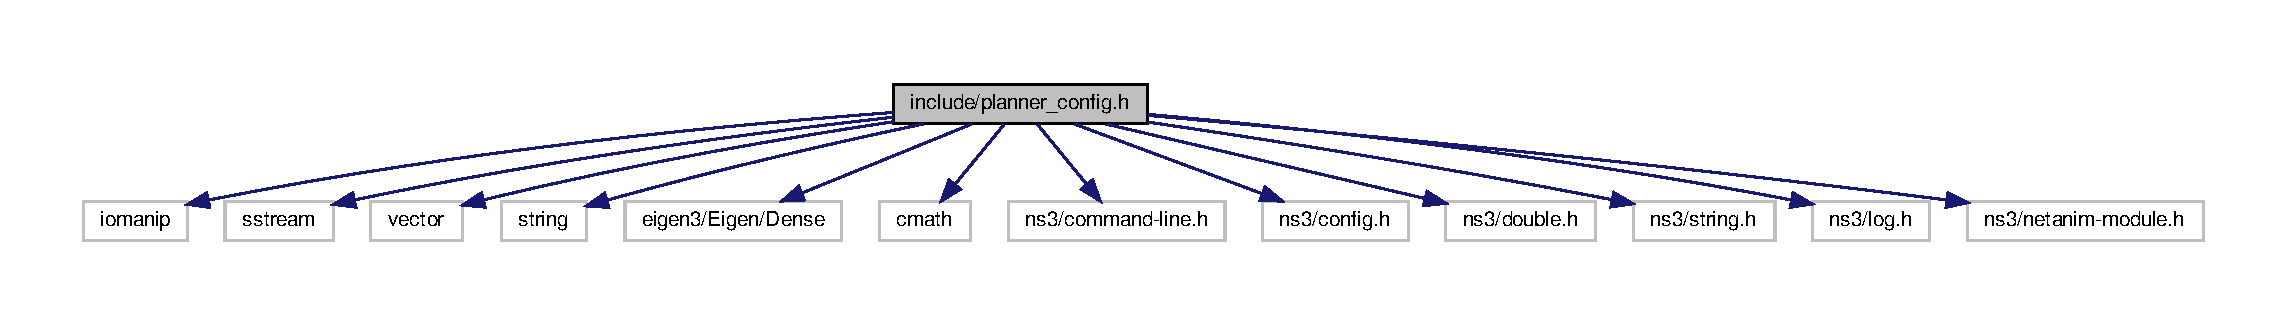
\includegraphics[width=350pt]{planner__config_8h__incl}
\end{center}
\end{figure}
This graph shows which files directly or indirectly include this file\+:
\nopagebreak
\begin{figure}[H]
\begin{center}
\leavevmode
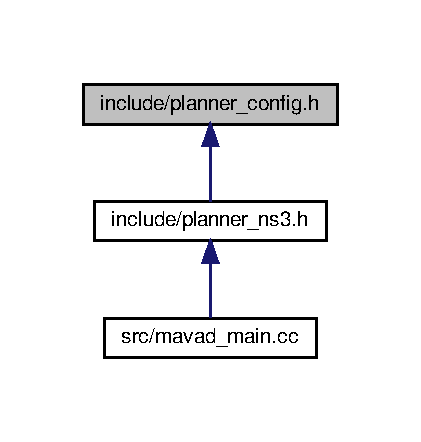
\includegraphics[width=202pt]{planner__config_8h__dep__incl}
\end{center}
\end{figure}
\subsection*{Classes}
\begin{DoxyCompactItemize}
\item 
struct \hyperlink{structrnl_1_1Nbt}{rnl\+::\+Nbt}
\begin{DoxyCompactList}\small\item\em For parsing and serializing data of neighbouring nodes. \end{DoxyCompactList}\item 
struct \hyperlink{structrnl_1_1USMsg}{rnl\+::\+U\+S\+Msg}
\begin{DoxyCompactList}\small\item\em This Structure Will be Serialized and sent as Unicast Message. The ~\newline
communication will have this format. Each drone sends ~\newline
Unicast Message in this format. The serializer will make a ~\newline
delimiter seperated string which will be passed onto the sockets ~\newline
for transmission. ~\newline
. \end{DoxyCompactList}\item 
struct \hyperlink{structrnl_1_1URMsg}{rnl\+::\+U\+R\+Msg}
\begin{DoxyCompactList}\small\item\em This Structure Will be parsed as a Unicast Message. The ~\newline
communication will have this format. Each drone receives ~\newline
Unicast Message in this format. The parser will convert ~\newline
the received message into struct members. ~\newline
. \end{DoxyCompactList}\end{DoxyCompactItemize}
\subsection*{Enumerations}
\begin{DoxyCompactItemize}
\item 
enum \hyperlink{planner__config_8h_abf2bd8ba1ccd0fa681ac5299ba19b5a1}{rnl\+::state} \{ \newline
\hyperlink{planner__config_8h_abf2bd8ba1ccd0fa681ac5299ba19b5a1a685c2f7e7e26cde40654a6c1e250e77e}{rnl\+::\+S\+F\+I\+R\+E\+D\+ET} = 1, 
\hyperlink{planner__config_8h_abf2bd8ba1ccd0fa681ac5299ba19b5a1aa17489432550b74b4ef15b52a2ae62b6}{rnl\+::\+S\+O\+N\+L\+I\+NE} = 2, 
\hyperlink{planner__config_8h_abf2bd8ba1ccd0fa681ac5299ba19b5a1ae25aa39ab558f3d0c434a4730db6da69}{rnl\+::\+S\+A\+N\+C\+H\+O\+R\+I\+NG} = 4, 
\hyperlink{planner__config_8h_abf2bd8ba1ccd0fa681ac5299ba19b5a1a1bc28766fabeea139725b605a6875847}{rnl\+::\+S\+L\+A\+N\+D\+U\+N\+A\+RM} = 8, 
\newline
\hyperlink{planner__config_8h_abf2bd8ba1ccd0fa681ac5299ba19b5a1a9f1612c2790d6547e2b4ed5dc588cdbd}{rnl\+::\+S\+G\+F\+I\+R\+E\+D\+ET} = 16, 
\hyperlink{planner__config_8h_abf2bd8ba1ccd0fa681ac5299ba19b5a1a76bfa4a4d798f385d4ed674c8d06d1c2}{rnl\+::\+S\+G\+D\+R\+O\+N\+E\+R\+EQ} = 32
 \}
\item 
\mbox{\Hypertarget{planner__config_8h_ab381da0fa5692e394ced69fc7155486e}\label{planner__config_8h_ab381da0fa5692e394ced69fc7155486e}} 
enum {\bfseries control} \{ \newline
{\bfseries C\+L\+A\+N\+D\+U\+N\+A\+RM} = 1, 
{\bfseries C\+H\+O\+L\+D\+RC} = 2, 
{\bfseries C\+C\+H\+A\+N\+G\+E\+P\+AR} = 4, 
{\bfseries C\+L\+T\+OP} = 8, 
\newline
{\bfseries C\+R\+T\+OP} = 16, 
{\bfseries C\+A\+T\+OP} = 32, 
{\bfseries C\+R\+ES} = 64
 \}
\end{DoxyCompactItemize}
\subsection*{Variables}
\begin{DoxyCompactItemize}
\item 
\mbox{\Hypertarget{planner__config_8h_ab0985dce78c6ca4a58ae60725c0999b1}\label{planner__config_8h_ab0985dce78c6ca4a58ae60725c0999b1}} 
static std\+::string {\bfseries rnl\+::\+D\+E\+L\+IM} = \char`\"{}\textbackslash{}n\char`\"{}
\item 
static std\+::string \hyperlink{planner__config_8h_a33c64a0043c93458fac36fe41a17aa8d}{rnl\+::\+D\+E\+L\+I\+M\+\_\+\+N\+B\+T\+H\+OP} = \char`\"{}$\vert$\char`\"{}
\item 
static std\+::string \hyperlink{planner__config_8h_a5aa5dac37bf587ab7a829ea362878baf}{rnl\+::\+D\+E\+L\+I\+M\+\_\+\+N\+B\+T\+P\+OS} = \char`\"{}.\char`\"{}
\item 
static std\+::string \hyperlink{planner__config_8h_a4c25161b0c28b01fef9be6ff225760d7}{rnl\+::\+D\+E\+L\+I\+M\+\_\+\+N\+B\+T\+I\+D\+\_\+\+P\+OS} = \char`\"{},\char`\"{}
\item 
static std\+::string \hyperlink{planner__config_8h_aaaa9f6bd2425ab763f939cd6e732fc7b}{rnl\+::\+D\+E\+L\+I\+M\+\_\+\+N\+B\+T\+M\+H\+OP} = \char`\"{}$\sim$$\sim$\char`\"{}
\item 
static std\+::string \hyperlink{planner__config_8h_a341e92a73f6f1fc6a1b50a1d2ce02263}{rnl\+::\+D\+E\+L\+I\+M\+\_\+\+P\+OS} = \char`\"{}\+:\char`\"{}
\item 
static std\+::string \hyperlink{planner__config_8h_a65876a0479b37a1a0388205ac257c0d0}{rnl\+::\+I\+P\+\_\+\+B\+A\+SE} = \char`\"{}10.\+1.\+1.\char`\"{}
\item 
static int \hyperlink{planner__config_8h_adf0cba08baeee1c91aed8ea4db125cb2}{rnl\+::\+B\+A\+S\+E\+ID} = 50
\item 
static double \hyperlink{planner__config_8h_a07c857b1b38dd2525bef4652da745681}{rnl\+::\+S\+T\+EP} = 0.\+5
\item 
static double \hyperlink{planner__config_8h_a3b98891dcbe5a105fa7806c23597b295}{rnl\+::\+RC} = 30.\+0
\item 
static double \hyperlink{planner__config_8h_a03a389b87a6cb32f5fd383083a3cbcd6}{rnl\+::\+D\+T\+H\+E\+TA} = rnl\+::\+S\+T\+EP / rnl\+::\+RC
\item 
static double \hyperlink{planner__config_8h_a6b8eceb57d0c8d8142e3fa840cebbed9}{rnl\+::\+M\+A\+X\+T\+H\+R\+E\+S\+H\+RC} = 100.\+0
\item 
static double \hyperlink{planner__config_8h_a18ac368908261271d2045e987956e809}{rnl\+::\+M\+I\+N\+T\+H\+R\+E\+S\+H\+RC} = 3.\+0
\end{DoxyCompactItemize}


\subsection{Detailed Description}
Configuration file for setting the serializing \& parsing of ns3 data to other formats. Contains the datatype for data encoding \& decoding and other static data variables. 

\begin{DoxyAuthor}{Author}
Ojit Mehta (\href{mailto:f20170372@goa.bits-pilani.ac.in}{\tt f20170372@goa.\+bits-\/pilani.\+ac.\+in}) 
\end{DoxyAuthor}
\begin{DoxyVersion}{Version}
0.\+1 
\end{DoxyVersion}
\begin{DoxyDate}{Date}
2021-\/03-\/29
\end{DoxyDate}
\begin{DoxyCopyright}{Copyright}
Copyright (c) 2021 
\end{DoxyCopyright}


\subsection{Enumeration Type Documentation}
\mbox{\Hypertarget{planner__config_8h_file_abf2bd8ba1ccd0fa681ac5299ba19b5a1}\label{planner__config_8h_file_abf2bd8ba1ccd0fa681ac5299ba19b5a1}} 
\index{planner\+\_\+config.\+h@{planner\+\_\+config.\+h}!state@{state}}
\index{state@{state}!planner\+\_\+config.\+h@{planner\+\_\+config.\+h}}
\subsubsection{\texorpdfstring{state}{state}}
{\footnotesize\ttfamily enum \hyperlink{planner__config_8h_abf2bd8ba1ccd0fa681ac5299ba19b5a1}{rnl\+::state}}

\begin{DoxyEnumFields}{Enumerator}
\raisebox{\heightof{T}}[0pt][0pt]{\index{S\+F\+I\+R\+E\+D\+ET@{S\+F\+I\+R\+E\+D\+ET}!planner\+\_\+config.\+h@{planner\+\_\+config.\+h}}\index{planner\+\_\+config.\+h@{planner\+\_\+config.\+h}!S\+F\+I\+R\+E\+D\+ET@{S\+F\+I\+R\+E\+D\+ET}}}\mbox{\Hypertarget{planner__config_8h_abf2bd8ba1ccd0fa681ac5299ba19b5a1a685c2f7e7e26cde40654a6c1e250e77e}\label{planner__config_8h_abf2bd8ba1ccd0fa681ac5299ba19b5a1a685c2f7e7e26cde40654a6c1e250e77e}} 
S\+F\+I\+R\+E\+D\+ET&\mbox{[}L\+O\+C\+AL S\+T\+A\+TE\mbox{]} State mentions fire detected by the system \\
\hline

\raisebox{\heightof{T}}[0pt][0pt]{\index{S\+O\+N\+L\+I\+NE@{S\+O\+N\+L\+I\+NE}!planner\+\_\+config.\+h@{planner\+\_\+config.\+h}}\index{planner\+\_\+config.\+h@{planner\+\_\+config.\+h}!S\+O\+N\+L\+I\+NE@{S\+O\+N\+L\+I\+NE}}}\mbox{\Hypertarget{planner__config_8h_abf2bd8ba1ccd0fa681ac5299ba19b5a1aa17489432550b74b4ef15b52a2ae62b6}\label{planner__config_8h_abf2bd8ba1ccd0fa681ac5299ba19b5a1aa17489432550b74b4ef15b52a2ae62b6}} 
S\+O\+N\+L\+I\+NE&\mbox{[}L\+O\+C\+AL S\+T\+A\+TE\mbox{]} Node is active \\
\hline

\raisebox{\heightof{T}}[0pt][0pt]{\index{S\+A\+N\+C\+H\+O\+R\+I\+NG@{S\+A\+N\+C\+H\+O\+R\+I\+NG}!planner\+\_\+config.\+h@{planner\+\_\+config.\+h}}\index{planner\+\_\+config.\+h@{planner\+\_\+config.\+h}!S\+A\+N\+C\+H\+O\+R\+I\+NG@{S\+A\+N\+C\+H\+O\+R\+I\+NG}}}\mbox{\Hypertarget{planner__config_8h_abf2bd8ba1ccd0fa681ac5299ba19b5a1ae25aa39ab558f3d0c434a4730db6da69}\label{planner__config_8h_abf2bd8ba1ccd0fa681ac5299ba19b5a1ae25aa39ab558f3d0c434a4730db6da69}} 
S\+A\+N\+C\+H\+O\+R\+I\+NG&\mbox{[}L\+O\+C\+AL S\+T\+A\+TE\mbox{]} Node is anchoring a node \\
\hline

\raisebox{\heightof{T}}[0pt][0pt]{\index{S\+L\+A\+N\+D\+U\+N\+A\+RM@{S\+L\+A\+N\+D\+U\+N\+A\+RM}!planner\+\_\+config.\+h@{planner\+\_\+config.\+h}}\index{planner\+\_\+config.\+h@{planner\+\_\+config.\+h}!S\+L\+A\+N\+D\+U\+N\+A\+RM@{S\+L\+A\+N\+D\+U\+N\+A\+RM}}}\mbox{\Hypertarget{planner__config_8h_abf2bd8ba1ccd0fa681ac5299ba19b5a1a1bc28766fabeea139725b605a6875847}\label{planner__config_8h_abf2bd8ba1ccd0fa681ac5299ba19b5a1a1bc28766fabeea139725b605a6875847}} 
S\+L\+A\+N\+D\+U\+N\+A\+RM&\mbox{[}L\+O\+C\+AL S\+T\+A\+TE\mbox{]} Node is inactive \\
\hline

\raisebox{\heightof{T}}[0pt][0pt]{\index{S\+G\+F\+I\+R\+E\+D\+ET@{S\+G\+F\+I\+R\+E\+D\+ET}!planner\+\_\+config.\+h@{planner\+\_\+config.\+h}}\index{planner\+\_\+config.\+h@{planner\+\_\+config.\+h}!S\+G\+F\+I\+R\+E\+D\+ET@{S\+G\+F\+I\+R\+E\+D\+ET}}}\mbox{\Hypertarget{planner__config_8h_abf2bd8ba1ccd0fa681ac5299ba19b5a1a9f1612c2790d6547e2b4ed5dc588cdbd}\label{planner__config_8h_abf2bd8ba1ccd0fa681ac5299ba19b5a1a9f1612c2790d6547e2b4ed5dc588cdbd}} 
S\+G\+F\+I\+R\+E\+D\+ET&\mbox{[}G\+L\+O\+B\+AL S\+T\+A\+TE\mbox{]} Swarm has detected fire \\
\hline

\raisebox{\heightof{T}}[0pt][0pt]{\index{S\+G\+D\+R\+O\+N\+E\+R\+EQ@{S\+G\+D\+R\+O\+N\+E\+R\+EQ}!planner\+\_\+config.\+h@{planner\+\_\+config.\+h}}\index{planner\+\_\+config.\+h@{planner\+\_\+config.\+h}!S\+G\+D\+R\+O\+N\+E\+R\+EQ@{S\+G\+D\+R\+O\+N\+E\+R\+EQ}}}\mbox{\Hypertarget{planner__config_8h_abf2bd8ba1ccd0fa681ac5299ba19b5a1a76bfa4a4d798f385d4ed674c8d06d1c2}\label{planner__config_8h_abf2bd8ba1ccd0fa681ac5299ba19b5a1a76bfa4a4d798f385d4ed674c8d06d1c2}} 
S\+G\+D\+R\+O\+N\+E\+R\+EQ&\mbox{[}G\+L\+O\+B\+AL S\+T\+A\+TE\mbox{]} Swarm asking for more drones \\
\hline

\end{DoxyEnumFields}


\subsection{Variable Documentation}
\mbox{\Hypertarget{planner__config_8h_file_adf0cba08baeee1c91aed8ea4db125cb2}\label{planner__config_8h_file_adf0cba08baeee1c91aed8ea4db125cb2}} 
\index{planner\+\_\+config.\+h@{planner\+\_\+config.\+h}!B\+A\+S\+E\+ID@{B\+A\+S\+E\+ID}}
\index{B\+A\+S\+E\+ID@{B\+A\+S\+E\+ID}!planner\+\_\+config.\+h@{planner\+\_\+config.\+h}}
\subsubsection{\texorpdfstring{B\+A\+S\+E\+ID}{BASEID}}
{\footnotesize\ttfamily int rnl\+::\+B\+A\+S\+E\+ID = 50\hspace{0.3cm}{\ttfamily [static]}}

IP Base \mbox{\Hypertarget{planner__config_8h_file_a33c64a0043c93458fac36fe41a17aa8d}\label{planner__config_8h_file_a33c64a0043c93458fac36fe41a17aa8d}} 
\index{planner\+\_\+config.\+h@{planner\+\_\+config.\+h}!D\+E\+L\+I\+M\+\_\+\+N\+B\+T\+H\+OP@{D\+E\+L\+I\+M\+\_\+\+N\+B\+T\+H\+OP}}
\index{D\+E\+L\+I\+M\+\_\+\+N\+B\+T\+H\+OP@{D\+E\+L\+I\+M\+\_\+\+N\+B\+T\+H\+OP}!planner\+\_\+config.\+h@{planner\+\_\+config.\+h}}
\subsubsection{\texorpdfstring{D\+E\+L\+I\+M\+\_\+\+N\+B\+T\+H\+OP}{DELIM\_NBTHOP}}
{\footnotesize\ttfamily std\+::string rnl\+::\+D\+E\+L\+I\+M\+\_\+\+N\+B\+T\+H\+OP = \char`\"{}$\vert$\char`\"{}\hspace{0.3cm}{\ttfamily [static]}}

Delimiter used for serializing message to stringstream \begin{DoxySeeAlso}{See also}
\hyperlink{structrnl_1_1USMsg_ad940de5a03b2ad545557cf202591df5c}{rnl\+::\+U\+S\+Msg\+::serialize()} 

U\+R\+Msg\+::serialize() 
\end{DoxySeeAlso}
\mbox{\Hypertarget{planner__config_8h_file_a4c25161b0c28b01fef9be6ff225760d7}\label{planner__config_8h_file_a4c25161b0c28b01fef9be6ff225760d7}} 
\index{planner\+\_\+config.\+h@{planner\+\_\+config.\+h}!D\+E\+L\+I\+M\+\_\+\+N\+B\+T\+I\+D\+\_\+\+P\+OS@{D\+E\+L\+I\+M\+\_\+\+N\+B\+T\+I\+D\+\_\+\+P\+OS}}
\index{D\+E\+L\+I\+M\+\_\+\+N\+B\+T\+I\+D\+\_\+\+P\+OS@{D\+E\+L\+I\+M\+\_\+\+N\+B\+T\+I\+D\+\_\+\+P\+OS}!planner\+\_\+config.\+h@{planner\+\_\+config.\+h}}
\subsubsection{\texorpdfstring{D\+E\+L\+I\+M\+\_\+\+N\+B\+T\+I\+D\+\_\+\+P\+OS}{DELIM\_NBTID\_POS}}
{\footnotesize\ttfamily std\+::string rnl\+::\+D\+E\+L\+I\+M\+\_\+\+N\+B\+T\+I\+D\+\_\+\+P\+OS = \char`\"{},\char`\"{}\hspace{0.3cm}{\ttfamily [static]}}

Delimiter for specifiying neighbouring hops \begin{DoxySeeAlso}{See also}
Nbt\+::serialize 
\end{DoxySeeAlso}
\mbox{\Hypertarget{planner__config_8h_file_aaaa9f6bd2425ab763f939cd6e732fc7b}\label{planner__config_8h_file_aaaa9f6bd2425ab763f939cd6e732fc7b}} 
\index{planner\+\_\+config.\+h@{planner\+\_\+config.\+h}!D\+E\+L\+I\+M\+\_\+\+N\+B\+T\+M\+H\+OP@{D\+E\+L\+I\+M\+\_\+\+N\+B\+T\+M\+H\+OP}}
\index{D\+E\+L\+I\+M\+\_\+\+N\+B\+T\+M\+H\+OP@{D\+E\+L\+I\+M\+\_\+\+N\+B\+T\+M\+H\+OP}!planner\+\_\+config.\+h@{planner\+\_\+config.\+h}}
\subsubsection{\texorpdfstring{D\+E\+L\+I\+M\+\_\+\+N\+B\+T\+M\+H\+OP}{DELIM\_NBTMHOP}}
{\footnotesize\ttfamily std\+::string rnl\+::\+D\+E\+L\+I\+M\+\_\+\+N\+B\+T\+M\+H\+OP = \char`\"{}$\sim$$\sim$\char`\"{}\hspace{0.3cm}{\ttfamily [static]}}

Delimiter for specifiying neighbouring hops \begin{DoxySeeAlso}{See also}
Nbt\+::serialize 
\end{DoxySeeAlso}
\mbox{\Hypertarget{planner__config_8h_file_a5aa5dac37bf587ab7a829ea362878baf}\label{planner__config_8h_file_a5aa5dac37bf587ab7a829ea362878baf}} 
\index{planner\+\_\+config.\+h@{planner\+\_\+config.\+h}!D\+E\+L\+I\+M\+\_\+\+N\+B\+T\+P\+OS@{D\+E\+L\+I\+M\+\_\+\+N\+B\+T\+P\+OS}}
\index{D\+E\+L\+I\+M\+\_\+\+N\+B\+T\+P\+OS@{D\+E\+L\+I\+M\+\_\+\+N\+B\+T\+P\+OS}!planner\+\_\+config.\+h@{planner\+\_\+config.\+h}}
\subsubsection{\texorpdfstring{D\+E\+L\+I\+M\+\_\+\+N\+B\+T\+P\+OS}{DELIM\_NBTPOS}}
{\footnotesize\ttfamily std\+::string rnl\+::\+D\+E\+L\+I\+M\+\_\+\+N\+B\+T\+P\+OS = \char`\"{}.\char`\"{}\hspace{0.3cm}{\ttfamily [static]}}

Delimiter for specifiying neighbouring hops \begin{DoxySeeAlso}{See also}
Nbt\+::serialize 
\end{DoxySeeAlso}
\mbox{\Hypertarget{planner__config_8h_file_a341e92a73f6f1fc6a1b50a1d2ce02263}\label{planner__config_8h_file_a341e92a73f6f1fc6a1b50a1d2ce02263}} 
\index{planner\+\_\+config.\+h@{planner\+\_\+config.\+h}!D\+E\+L\+I\+M\+\_\+\+P\+OS@{D\+E\+L\+I\+M\+\_\+\+P\+OS}}
\index{D\+E\+L\+I\+M\+\_\+\+P\+OS@{D\+E\+L\+I\+M\+\_\+\+P\+OS}!planner\+\_\+config.\+h@{planner\+\_\+config.\+h}}
\subsubsection{\texorpdfstring{D\+E\+L\+I\+M\+\_\+\+P\+OS}{DELIM\_POS}}
{\footnotesize\ttfamily std\+::string rnl\+::\+D\+E\+L\+I\+M\+\_\+\+P\+OS = \char`\"{}\+:\char`\"{}\hspace{0.3cm}{\ttfamily [static]}}

Delimiter seperating neighbours based on hop count \begin{DoxySeeAlso}{See also}
Nbt\+::serialize 
\end{DoxySeeAlso}
\mbox{\Hypertarget{planner__config_8h_file_a03a389b87a6cb32f5fd383083a3cbcd6}\label{planner__config_8h_file_a03a389b87a6cb32f5fd383083a3cbcd6}} 
\index{planner\+\_\+config.\+h@{planner\+\_\+config.\+h}!D\+T\+H\+E\+TA@{D\+T\+H\+E\+TA}}
\index{D\+T\+H\+E\+TA@{D\+T\+H\+E\+TA}!planner\+\_\+config.\+h@{planner\+\_\+config.\+h}}
\subsubsection{\texorpdfstring{D\+T\+H\+E\+TA}{DTHETA}}
{\footnotesize\ttfamily double rnl\+::\+D\+T\+H\+E\+TA = rnl\+::\+S\+T\+EP / rnl\+::\+RC\hspace{0.3cm}{\ttfamily [static]}}

RC Distance as specified in the paper. Ideal distance of seperation between two nodes \mbox{\Hypertarget{planner__config_8h_file_a65876a0479b37a1a0388205ac257c0d0}\label{planner__config_8h_file_a65876a0479b37a1a0388205ac257c0d0}} 
\index{planner\+\_\+config.\+h@{planner\+\_\+config.\+h}!I\+P\+\_\+\+B\+A\+SE@{I\+P\+\_\+\+B\+A\+SE}}
\index{I\+P\+\_\+\+B\+A\+SE@{I\+P\+\_\+\+B\+A\+SE}!planner\+\_\+config.\+h@{planner\+\_\+config.\+h}}
\subsubsection{\texorpdfstring{I\+P\+\_\+\+B\+A\+SE}{IP\_BASE}}
{\footnotesize\ttfamily std\+::string rnl\+::\+I\+P\+\_\+\+B\+A\+SE = \char`\"{}10.\+1.\+1.\char`\"{}\hspace{0.3cm}{\ttfamily [static]}}

Delimiter seperating coordinate value of robot pose \begin{DoxySeeAlso}{See also}
U\+R\+Msg\+::parse\+Unicast 
\end{DoxySeeAlso}
\mbox{\Hypertarget{planner__config_8h_file_a6b8eceb57d0c8d8142e3fa840cebbed9}\label{planner__config_8h_file_a6b8eceb57d0c8d8142e3fa840cebbed9}} 
\index{planner\+\_\+config.\+h@{planner\+\_\+config.\+h}!M\+A\+X\+T\+H\+R\+E\+S\+H\+RC@{M\+A\+X\+T\+H\+R\+E\+S\+H\+RC}}
\index{M\+A\+X\+T\+H\+R\+E\+S\+H\+RC@{M\+A\+X\+T\+H\+R\+E\+S\+H\+RC}!planner\+\_\+config.\+h@{planner\+\_\+config.\+h}}
\subsubsection{\texorpdfstring{M\+A\+X\+T\+H\+R\+E\+S\+H\+RC}{MAXTHRESHRC}}
{\footnotesize\ttfamily double rnl\+::\+M\+A\+X\+T\+H\+R\+E\+S\+H\+RC = 100.\+0\hspace{0.3cm}{\ttfamily [static]}}

Max dtheta that a drone can undertake at a particular time \mbox{\Hypertarget{planner__config_8h_file_a18ac368908261271d2045e987956e809}\label{planner__config_8h_file_a18ac368908261271d2045e987956e809}} 
\index{planner\+\_\+config.\+h@{planner\+\_\+config.\+h}!M\+I\+N\+T\+H\+R\+E\+S\+H\+RC@{M\+I\+N\+T\+H\+R\+E\+S\+H\+RC}}
\index{M\+I\+N\+T\+H\+R\+E\+S\+H\+RC@{M\+I\+N\+T\+H\+R\+E\+S\+H\+RC}!planner\+\_\+config.\+h@{planner\+\_\+config.\+h}}
\subsubsection{\texorpdfstring{M\+I\+N\+T\+H\+R\+E\+S\+H\+RC}{MINTHRESHRC}}
{\footnotesize\ttfamily double rnl\+::\+M\+I\+N\+T\+H\+R\+E\+S\+H\+RC = 3.\+0\hspace{0.3cm}{\ttfamily [static]}}

Maximum RC threshold for 2 nodes to communicate \mbox{\Hypertarget{planner__config_8h_file_a3b98891dcbe5a105fa7806c23597b295}\label{planner__config_8h_file_a3b98891dcbe5a105fa7806c23597b295}} 
\index{planner\+\_\+config.\+h@{planner\+\_\+config.\+h}!RC@{RC}}
\index{RC@{RC}!planner\+\_\+config.\+h@{planner\+\_\+config.\+h}}
\subsubsection{\texorpdfstring{RC}{RC}}
{\footnotesize\ttfamily double rnl\+::\+RC = 30.\+0\hspace{0.3cm}{\ttfamily [static]}}

Step Size for discretizing \mbox{\Hypertarget{planner__config_8h_file_a07c857b1b38dd2525bef4652da745681}\label{planner__config_8h_file_a07c857b1b38dd2525bef4652da745681}} 
\index{planner\+\_\+config.\+h@{planner\+\_\+config.\+h}!S\+T\+EP@{S\+T\+EP}}
\index{S\+T\+EP@{S\+T\+EP}!planner\+\_\+config.\+h@{planner\+\_\+config.\+h}}
\subsubsection{\texorpdfstring{S\+T\+EP}{STEP}}
{\footnotesize\ttfamily double rnl\+::\+S\+T\+EP = 0.\+5\hspace{0.3cm}{\ttfamily [static]}}

Base Station IP Address 
\hypertarget{planner__ns3_8h}{}\section{include/planner\+\_\+ns3.h File Reference}
\label{planner__ns3_8h}\index{include/planner\+\_\+ns3.\+h@{include/planner\+\_\+ns3.\+h}}


Planner class for the project.  


{\ttfamily \#include \char`\"{}planner\+\_\+config.\+h\char`\"{}}\newline
{\ttfamily \#include \char`\"{}planner\+\_\+ns3\+\_\+utils.\+h\char`\"{}}\newline
{\ttfamily \#include \char`\"{}ns3/core-\/module.\+h\char`\"{}}\newline
{\ttfamily \#include $<$cmath$>$}\newline
{\ttfamily \#include \char`\"{}ns3/command-\/line.\+h\char`\"{}}\newline
{\ttfamily \#include \char`\"{}ns3/config.\+h\char`\"{}}\newline
{\ttfamily \#include \char`\"{}ns3/double.\+h\char`\"{}}\newline
{\ttfamily \#include \char`\"{}ns3/string.\+h\char`\"{}}\newline
{\ttfamily \#include \char`\"{}ns3/log.\+h\char`\"{}}\newline
{\ttfamily \#include \char`\"{}ns3/yans-\/wifi-\/helper.\+h\char`\"{}}\newline
{\ttfamily \#include \char`\"{}ns3/mobility-\/helper.\+h\char`\"{}}\newline
{\ttfamily \#include \char`\"{}ns3/ipv4-\/address-\/helper.\+h\char`\"{}}\newline
{\ttfamily \#include \char`\"{}ns3/yans-\/wifi-\/channel.\+h\char`\"{}}\newline
{\ttfamily \#include \char`\"{}ns3/mobility-\/model.\+h\char`\"{}}\newline
{\ttfamily \#include \char`\"{}ns3/internet-\/stack-\/helper.\+h\char`\"{}}\newline
{\ttfamily \#include \char`\"{}ns3/netanim-\/module.\+h\char`\"{}}\newline
Include dependency graph for planner\+\_\+ns3.\+h\+:\nopagebreak
\begin{figure}[H]
\begin{center}
\leavevmode
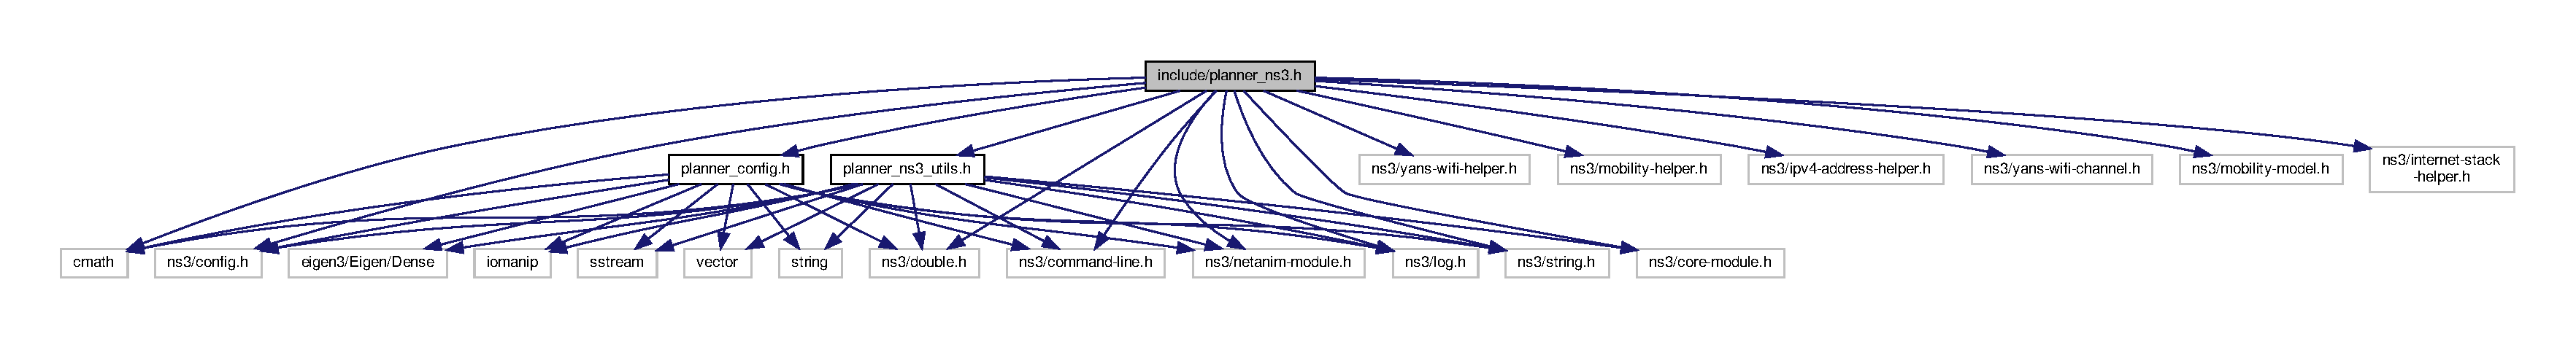
\includegraphics[width=350pt]{planner__ns3_8h__incl}
\end{center}
\end{figure}
This graph shows which files directly or indirectly include this file\+:\nopagebreak
\begin{figure}[H]
\begin{center}
\leavevmode
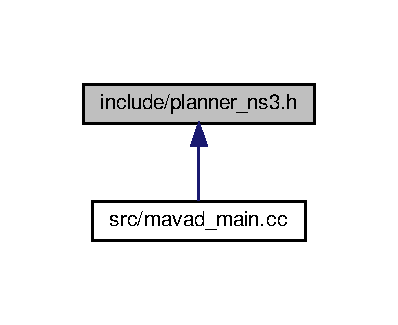
\includegraphics[width=191pt]{planner__ns3_8h__dep__incl}
\end{center}
\end{figure}
\subsection*{Classes}
\begin{DoxyCompactItemize}
\item 
struct \hyperlink{structrnl_1_1DroneSoc}{rnl\+::\+Drone\+Soc}
\begin{DoxyCompactList}\small\item\em Drone Socket common for planning and communication. \end{DoxyCompactList}\item 
class \hyperlink{classrnl_1_1Properties}{rnl\+::\+Properties}
\item 
class \hyperlink{classrnl_1_1Planner}{rnl\+::\+Planner}
\begin{DoxyCompactList}\small\item\em \hyperlink{classrnl_1_1Planner}{Planner} class. Flow ~\newline
. \end{DoxyCompactList}\end{DoxyCompactItemize}
\subsection*{Functions}
\begin{DoxyCompactItemize}
\item 
\hyperlink{structrnl_1_1Nbt}{rnl\+::\+Nbt} \hyperlink{planner__ns3_8h_a596f93e58e27735e9a8ea3bf7fbdaeff}{rnl\+::setinitial\+Nbt} (int id, int n)
\begin{DoxyCompactList}\small\item\em Initial neighbour table to be set. Since we are initializing the nodes in linear fashion ~\newline
 Setting it requires only index of the node. ~\newline
Set to id + 1 and id -\/ 1 as one hop neighbours. \end{DoxyCompactList}\item 
\hyperlink{structrnl_1_1USMsg}{rnl\+::\+U\+S\+Msg} \hyperlink{planner__ns3_8h_ac76d8dd7ac6e2dfe7034c65e0b9e08d9}{rnl\+::setinitial\+S\+Msg} (\hyperlink{structrnl_1_1Nbt}{rnl\+::\+Nbt} nbt, int id, int n)
\begin{DoxyCompactList}\small\item\em Set the initial message to be sent to successor. \end{DoxyCompactList}\end{DoxyCompactItemize}


\subsection{Detailed Description}
Planner class for the project. 

\begin{DoxyAuthor}{Author}
Ojit Mehta (\href{mailto:f20170372@goa.bits-pilani.ac.in}{\tt f20170372@goa.\+bits-\/pilani.\+ac.\+in}) 
\end{DoxyAuthor}
\begin{DoxyVersion}{Version}
0.\+1 
\end{DoxyVersion}
\begin{DoxyDate}{Date}
2021-\/04-\/05
\end{DoxyDate}
\begin{DoxyCopyright}{Copyright}
Copyright (c) 2021 
\end{DoxyCopyright}


\subsection{Function Documentation}
\mbox{\Hypertarget{planner__ns3_8h_file_a596f93e58e27735e9a8ea3bf7fbdaeff}\label{planner__ns3_8h_file_a596f93e58e27735e9a8ea3bf7fbdaeff}} 
\index{planner\+\_\+ns3.\+h@{planner\+\_\+ns3.\+h}!setinitial\+Nbt@{setinitial\+Nbt}}
\index{setinitial\+Nbt@{setinitial\+Nbt}!planner\+\_\+ns3.\+h@{planner\+\_\+ns3.\+h}}
\subsubsection{\texorpdfstring{setinitial\+Nbt()}{setinitialNbt()}}
{\footnotesize\ttfamily \hyperlink{structrnl_1_1Nbt}{rnl\+::\+Nbt} rnl\+::setinitial\+Nbt (\begin{DoxyParamCaption}\item[{int}]{id,  }\item[{int}]{n }\end{DoxyParamCaption})}



Initial neighbour table to be set. Since we are initializing the nodes in linear fashion ~\newline
 Setting it requires only index of the node. ~\newline
Set to id + 1 and id -\/ 1 as one hop neighbours. 


\begin{DoxyParams}{Parameters}
{\em id} & Index \\
\hline
{\em n} & number of nodes \\
\hline
\end{DoxyParams}
\begin{DoxyReturn}{Returns}
\hyperlink{structrnl_1_1Nbt}{rnl\+::\+Nbt} 
\end{DoxyReturn}
\mbox{\Hypertarget{planner__ns3_8h_file_ac76d8dd7ac6e2dfe7034c65e0b9e08d9}\label{planner__ns3_8h_file_ac76d8dd7ac6e2dfe7034c65e0b9e08d9}} 
\index{planner\+\_\+ns3.\+h@{planner\+\_\+ns3.\+h}!setinitial\+S\+Msg@{setinitial\+S\+Msg}}
\index{setinitial\+S\+Msg@{setinitial\+S\+Msg}!planner\+\_\+ns3.\+h@{planner\+\_\+ns3.\+h}}
\subsubsection{\texorpdfstring{setinitial\+S\+Msg()}{setinitialSMsg()}}
{\footnotesize\ttfamily \hyperlink{structrnl_1_1USMsg}{rnl\+::\+U\+S\+Msg} rnl\+::setinitial\+S\+Msg (\begin{DoxyParamCaption}\item[{\hyperlink{structrnl_1_1Nbt}{rnl\+::\+Nbt}}]{nbt,  }\item[{int}]{id,  }\item[{int}]{n }\end{DoxyParamCaption})}



Set the initial message to be sent to successor. 


\begin{DoxyParams}{Parameters}
{\em nbt} & Initial neighbour table \\
\hline
{\em id} & Destination address sent to id + 1 \\
\hline
{\em n} & number number of nodes \\
\hline
\end{DoxyParams}
\begin{DoxyReturn}{Returns}
\hyperlink{structrnl_1_1USMsg}{rnl\+::\+U\+S\+Msg} 
\end{DoxyReturn}

\hypertarget{planner__ns3__utils_8h}{}\section{include/planner\+\_\+ns3\+\_\+utils.h File Reference}
\label{planner__ns3__utils_8h}\index{include/planner\+\_\+ns3\+\_\+utils.\+h@{include/planner\+\_\+ns3\+\_\+utils.\+h}}


Utility functions for Swarm Planner.  


{\ttfamily \#include $<$iomanip$>$}\newline
{\ttfamily \#include $<$sstream$>$}\newline
{\ttfamily \#include $<$vector$>$}\newline
{\ttfamily \#include $<$string$>$}\newline
{\ttfamily \#include $<$eigen3/\+Eigen/\+Dense$>$}\newline
{\ttfamily \#include $<$cmath$>$}\newline
{\ttfamily \#include \char`\"{}ns3/core-\/module.\+h\char`\"{}}\newline
{\ttfamily \#include \char`\"{}ns3/command-\/line.\+h\char`\"{}}\newline
{\ttfamily \#include \char`\"{}ns3/config.\+h\char`\"{}}\newline
{\ttfamily \#include \char`\"{}ns3/double.\+h\char`\"{}}\newline
{\ttfamily \#include \char`\"{}ns3/string.\+h\char`\"{}}\newline
{\ttfamily \#include \char`\"{}ns3/log.\+h\char`\"{}}\newline
{\ttfamily \#include \char`\"{}ns3/netanim-\/module.\+h\char`\"{}}\newline
Include dependency graph for planner\+\_\+ns3\+\_\+utils.\+h\+:\nopagebreak
\begin{figure}[H]
\begin{center}
\leavevmode
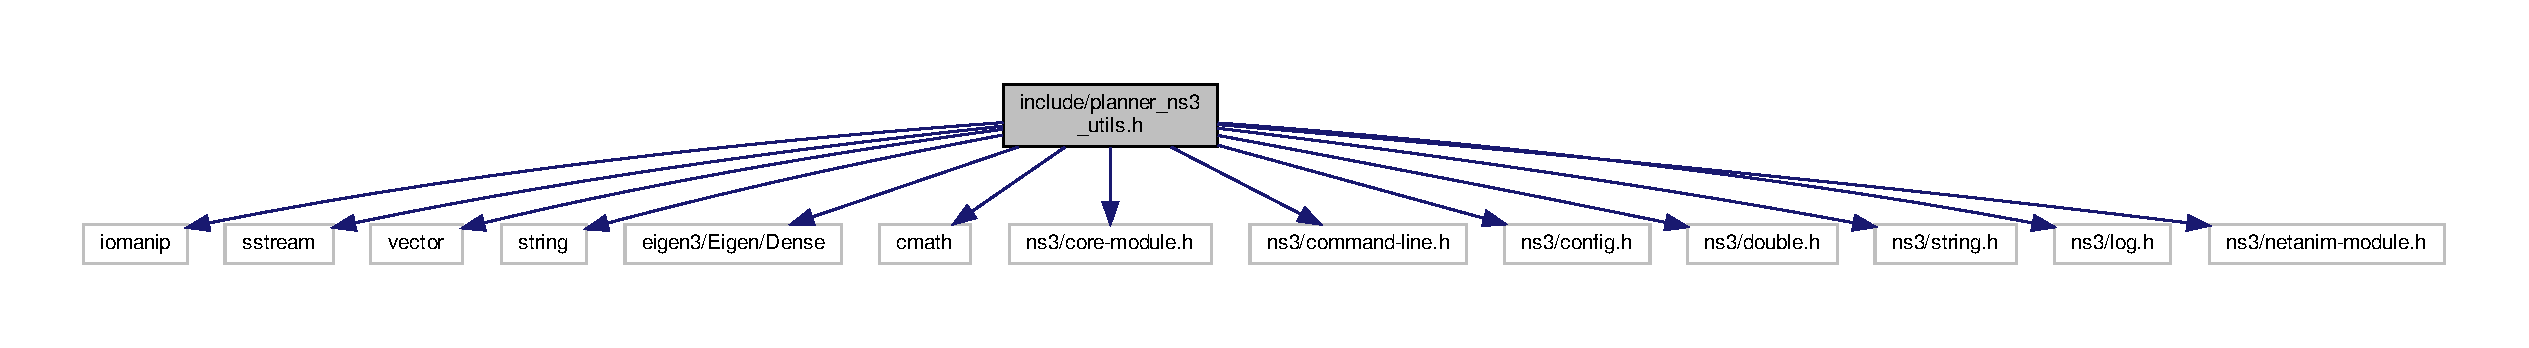
\includegraphics[width=350pt]{planner__ns3__utils_8h__incl}
\end{center}
\end{figure}
This graph shows which files directly or indirectly include this file\+:
\nopagebreak
\begin{figure}[H]
\begin{center}
\leavevmode
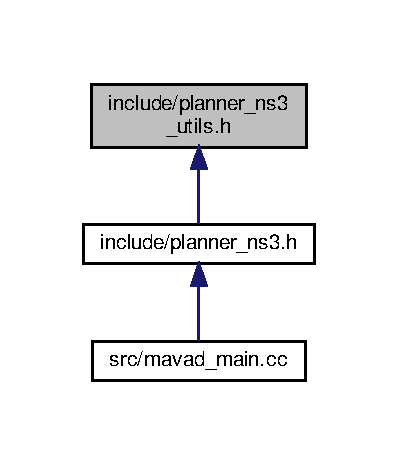
\includegraphics[width=191pt]{planner__ns3__utils_8h__dep__incl}
\end{center}
\end{figure}
\subsection*{Functions}
\begin{DoxyCompactItemize}
\item 
void \hyperlink{planner__ns3__utils_8h_af58ae6cb4570d154e757b71ea4c9ebe3}{rnl\+::set\+Position} (ns3\+::\+Ptr$<$ ns3\+::\+Node $>$ node, ns3\+::\+Vector3D pos)
\begin{DoxyCompactList}\small\item\em Set the Position of an ns3 node. \end{DoxyCompactList}\item 
ns3\+::\+Vector3D \hyperlink{planner__ns3__utils_8h_a04cf5f7c502bfec16c4c537de821216d}{rnl\+::get\+Position} (ns3\+::\+Ptr$<$ ns3\+::\+Node $>$ node)
\begin{DoxyCompactList}\small\item\em Get the Position object. \end{DoxyCompactList}\item 
bool \hyperlink{planner__ns3__utils_8h_a9279a10202a5c055d4b81a27dd288ee3}{rnl\+::get\+Trajectory} (std\+::vector$<$ ns3\+::\+Vector3D $>$ $\ast$wpts, ns3\+::\+Vector3D start\+\_\+pos, ns3\+::\+Vector3D end\+\_\+pos, double step)
\begin{DoxyCompactList}\small\item\em Get a Trajectory for U\+AV. \end{DoxyCompactList}\item 
bool \hyperlink{planner__ns3__utils_8h_af98d66186d02708f6f2e5c116a1334c2}{rnl\+::get\+Circlewpts} (std\+::vector$<$ ns3\+::\+Vector3D $>$ $\ast$wpts, ns3\+::\+Vector3D anch\+\_\+node, ns3\+::\+Vector3D child\+\_\+node, const float circle\+\_\+radius, const float dtheta, const int dir, const float step)
\begin{DoxyCompactList}\small\item\em Get Trajectory while in phase 2 of operation (Anchoring about a U\+AV) \end{DoxyCompactList}\item 
bool \hyperlink{planner__ns3__utils_8h_ad633f79350448ed52c934fe8ad2338fe}{rnl\+::get\+To\+Circle\+Range} (std\+::vector$<$ ns3\+::\+Vector3D $>$ $\ast$wpts, ns3\+::\+Vector3D \+\_\+anch\+\_\+p, ns3\+::\+Vector3D \+\_\+my\+\_\+p, float cr, float step)
\begin{DoxyCompactList}\small\item\em Get the To Circle Range object. \end{DoxyCompactList}\item 
float \hyperlink{planner__ns3__utils_8h_a061dbe3df5e23c8bbd49a7c87a65c392}{rnl\+::circling\+Offset} (ns3\+::\+Vector3D anch, ns3\+::\+Vector3D child, float \+\_\+cr)
\begin{DoxyCompactList}\small\item\em Offset to reach from child location to anchor location for getting to Circling radius of anchor. \end{DoxyCompactList}\item 
void \hyperlink{planner__ns3__utils_8h_a16545feffc1f0ba83c4ef72b6a5bb8c8}{rnl\+::pos\+Hold} (std\+::vector$<$ ns3\+::\+Vector3D $>$ $\ast$wpts, ns3\+::\+Vector3D pos)
\begin{DoxyCompactList}\small\item\em Waypoints passed for Position Hold requirement. \end{DoxyCompactList}\end{DoxyCompactItemize}


\subsection{Detailed Description}
Utility functions for Swarm Planner. 

\begin{DoxyAuthor}{Author}
Ojit Mehta (\href{mailto:f20170372@goa.bits-pilani.ac.in}{\tt f20170372@goa.\+bits-\/pilani.\+ac.\+in}) 
\end{DoxyAuthor}
\begin{DoxyVersion}{Version}
0.\+1 
\end{DoxyVersion}
\begin{DoxyDate}{Date}
2021-\/04-\/04
\end{DoxyDate}
\begin{DoxyCopyright}{Copyright}
Copyright (c) 2021 
\end{DoxyCopyright}


\subsection{Function Documentation}
\mbox{\Hypertarget{planner__ns3__utils_8h_file_a061dbe3df5e23c8bbd49a7c87a65c392}\label{planner__ns3__utils_8h_file_a061dbe3df5e23c8bbd49a7c87a65c392}} 
\index{planner\+\_\+ns3\+\_\+utils.\+h@{planner\+\_\+ns3\+\_\+utils.\+h}!circling\+Offset@{circling\+Offset}}
\index{circling\+Offset@{circling\+Offset}!planner\+\_\+ns3\+\_\+utils.\+h@{planner\+\_\+ns3\+\_\+utils.\+h}}
\subsubsection{\texorpdfstring{circling\+Offset()}{circlingOffset()}}
{\footnotesize\ttfamily float rnl\+::circling\+Offset (\begin{DoxyParamCaption}\item[{ns3\+::\+Vector3D}]{anch,  }\item[{ns3\+::\+Vector3D}]{child,  }\item[{float}]{\+\_\+cr }\end{DoxyParamCaption})}



Offset to reach from child location to anchor location for getting to Circling radius of anchor. 


\begin{DoxyParams}{Parameters}
{\em anch} & Anchor location \\
\hline
{\em child} & Child location \\
\hline
{\em \+\_\+cr} & Circling Radius \\
\hline
\end{DoxyParams}
\begin{DoxyReturn}{Returns}
float Offset returned 
\end{DoxyReturn}
\mbox{\Hypertarget{planner__ns3__utils_8h_file_af98d66186d02708f6f2e5c116a1334c2}\label{planner__ns3__utils_8h_file_af98d66186d02708f6f2e5c116a1334c2}} 
\index{planner\+\_\+ns3\+\_\+utils.\+h@{planner\+\_\+ns3\+\_\+utils.\+h}!get\+Circlewpts@{get\+Circlewpts}}
\index{get\+Circlewpts@{get\+Circlewpts}!planner\+\_\+ns3\+\_\+utils.\+h@{planner\+\_\+ns3\+\_\+utils.\+h}}
\subsubsection{\texorpdfstring{get\+Circlewpts()}{getCirclewpts()}}
{\footnotesize\ttfamily bool rnl\+::get\+Circlewpts (\begin{DoxyParamCaption}\item[{std\+::vector$<$ ns3\+::\+Vector3D $>$ $\ast$}]{wpts,  }\item[{ns3\+::\+Vector3D}]{anch\+\_\+node,  }\item[{ns3\+::\+Vector3D}]{child\+\_\+node,  }\item[{const float}]{circle\+\_\+radius,  }\item[{const float}]{dtheta,  }\item[{const int}]{dir,  }\item[{const float}]{step }\end{DoxyParamCaption})}



Get Trajectory while in phase 2 of operation (Anchoring about a U\+AV) 


\begin{DoxyParams}{Parameters}
{\em wpts} & Waypoints pointer to be filled by final trajectory locations \\
\hline
{\em anch\+\_\+node} & Location of anchoring node (Centre of the circle) \\
\hline
{\em child\+\_\+node} & current Location of child node (Start position) \\
\hline
{\em circle\+\_\+radius} & Radius at which waypoints need to be \\
\hline
{\em dtheta} & Theta increment at which waypoints need to be added \\
\hline
{\em dir} & Direction at which to increment (+ve Anticlockwise), (-\/ve Clockwise) \\
\hline
{\em step} & Step size used for getting to Circling Range of Anchoring node \\
\hline
\end{DoxyParams}
\begin{DoxyReturn}{Returns}
true if path found 

false if path not found 
\end{DoxyReturn}
\mbox{\Hypertarget{planner__ns3__utils_8h_file_a04cf5f7c502bfec16c4c537de821216d}\label{planner__ns3__utils_8h_file_a04cf5f7c502bfec16c4c537de821216d}} 
\index{planner\+\_\+ns3\+\_\+utils.\+h@{planner\+\_\+ns3\+\_\+utils.\+h}!get\+Position@{get\+Position}}
\index{get\+Position@{get\+Position}!planner\+\_\+ns3\+\_\+utils.\+h@{planner\+\_\+ns3\+\_\+utils.\+h}}
\subsubsection{\texorpdfstring{get\+Position()}{getPosition()}}
{\footnotesize\ttfamily ns3\+::\+Vector3D rnl\+::get\+Position (\begin{DoxyParamCaption}\item[{ns3\+::\+Ptr$<$ ns3\+::\+Node $>$}]{node }\end{DoxyParamCaption})}



Get the Position object. 


\begin{DoxyParams}{Parameters}
{\em node} & get the position of object at this node \\
\hline
\end{DoxyParams}
\begin{DoxyReturn}{Returns}
ns3\+::\+Vector3D 
\end{DoxyReturn}
\mbox{\Hypertarget{planner__ns3__utils_8h_file_ad633f79350448ed52c934fe8ad2338fe}\label{planner__ns3__utils_8h_file_ad633f79350448ed52c934fe8ad2338fe}} 
\index{planner\+\_\+ns3\+\_\+utils.\+h@{planner\+\_\+ns3\+\_\+utils.\+h}!get\+To\+Circle\+Range@{get\+To\+Circle\+Range}}
\index{get\+To\+Circle\+Range@{get\+To\+Circle\+Range}!planner\+\_\+ns3\+\_\+utils.\+h@{planner\+\_\+ns3\+\_\+utils.\+h}}
\subsubsection{\texorpdfstring{get\+To\+Circle\+Range()}{getToCircleRange()}}
{\footnotesize\ttfamily bool rnl\+::get\+To\+Circle\+Range (\begin{DoxyParamCaption}\item[{std\+::vector$<$ ns3\+::\+Vector3D $>$ $\ast$}]{wpts,  }\item[{ns3\+::\+Vector3D}]{\+\_\+anch\+\_\+p,  }\item[{ns3\+::\+Vector3D}]{\+\_\+my\+\_\+p,  }\item[{float}]{cr,  }\item[{float}]{step }\end{DoxyParamCaption})}



Get the To Circle Range object. 


\begin{DoxyParams}{Parameters}
{\em wpts} & Waypoints pointer to be filled by final trajectory locations \\
\hline
{\em \+\_\+anch\+\_\+p} & Anchor position \\
\hline
{\em \+\_\+my\+\_\+p} & Start Position \\
\hline
{\em cr} & Circling Radius required \\
\hline
{\em step} & Step size at which to add waypoints \\
\hline
\end{DoxyParams}
\begin{DoxyReturn}{Returns}
true if succeeded 

false if failed 
\end{DoxyReturn}
\mbox{\Hypertarget{planner__ns3__utils_8h_file_a9279a10202a5c055d4b81a27dd288ee3}\label{planner__ns3__utils_8h_file_a9279a10202a5c055d4b81a27dd288ee3}} 
\index{planner\+\_\+ns3\+\_\+utils.\+h@{planner\+\_\+ns3\+\_\+utils.\+h}!get\+Trajectory@{get\+Trajectory}}
\index{get\+Trajectory@{get\+Trajectory}!planner\+\_\+ns3\+\_\+utils.\+h@{planner\+\_\+ns3\+\_\+utils.\+h}}
\subsubsection{\texorpdfstring{get\+Trajectory()}{getTrajectory()}}
{\footnotesize\ttfamily bool rnl\+::get\+Trajectory (\begin{DoxyParamCaption}\item[{std\+::vector$<$ ns3\+::\+Vector3D $>$ $\ast$}]{wpts,  }\item[{ns3\+::\+Vector3D}]{start\+\_\+pos,  }\item[{ns3\+::\+Vector3D}]{end\+\_\+pos,  }\item[{double}]{step }\end{DoxyParamCaption})}



Get a Trajectory for U\+AV. 


\begin{DoxyParams}{Parameters}
{\em wpts} & Waypoints pointer to be filled by final trajectory locations \\
\hline
{\em start\+\_\+pos} & Starting position for the robot \\
\hline
{\em end\+\_\+pos} & Ending position for the robot \\
\hline
{\em step} & step size at which point seperation is required in the trajectory \\
\hline
\end{DoxyParams}
\begin{DoxyReturn}{Returns}
true if trajectory found 

false if no trajectory was found 
\end{DoxyReturn}
\mbox{\Hypertarget{planner__ns3__utils_8h_file_a16545feffc1f0ba83c4ef72b6a5bb8c8}\label{planner__ns3__utils_8h_file_a16545feffc1f0ba83c4ef72b6a5bb8c8}} 
\index{planner\+\_\+ns3\+\_\+utils.\+h@{planner\+\_\+ns3\+\_\+utils.\+h}!pos\+Hold@{pos\+Hold}}
\index{pos\+Hold@{pos\+Hold}!planner\+\_\+ns3\+\_\+utils.\+h@{planner\+\_\+ns3\+\_\+utils.\+h}}
\subsubsection{\texorpdfstring{pos\+Hold()}{posHold()}}
{\footnotesize\ttfamily void rnl\+::pos\+Hold (\begin{DoxyParamCaption}\item[{std\+::vector$<$ ns3\+::\+Vector3D $>$ $\ast$}]{wpts,  }\item[{ns3\+::\+Vector3D}]{pos }\end{DoxyParamCaption})}



Waypoints passed for Position Hold requirement. 


\begin{DoxyParams}{Parameters}
{\em wpts} & Waypoints pointer to be filled by final trajectory locations \\
\hline
{\em pos} & Position at which to hold position \\
\hline
\end{DoxyParams}
\mbox{\Hypertarget{planner__ns3__utils_8h_file_af58ae6cb4570d154e757b71ea4c9ebe3}\label{planner__ns3__utils_8h_file_af58ae6cb4570d154e757b71ea4c9ebe3}} 
\index{planner\+\_\+ns3\+\_\+utils.\+h@{planner\+\_\+ns3\+\_\+utils.\+h}!set\+Position@{set\+Position}}
\index{set\+Position@{set\+Position}!planner\+\_\+ns3\+\_\+utils.\+h@{planner\+\_\+ns3\+\_\+utils.\+h}}
\subsubsection{\texorpdfstring{set\+Position()}{setPosition()}}
{\footnotesize\ttfamily void rnl\+::set\+Position (\begin{DoxyParamCaption}\item[{ns3\+::\+Ptr$<$ ns3\+::\+Node $>$}]{node,  }\item[{ns3\+::\+Vector3D}]{pos }\end{DoxyParamCaption})}



Set the Position of an ns3 node. 


\begin{DoxyParams}{Parameters}
{\em node} & Node Pointer for which the position needs to be set \\
\hline
{\em pos} & position to set it to \\
\hline
\end{DoxyParams}

\hypertarget{mavad__main_8cc}{}\section{src/mavad\+\_\+main.cc File Reference}
\label{mavad__main_8cc}\index{src/mavad\+\_\+main.\+cc@{src/mavad\+\_\+main.\+cc}}


Exucatable file for simulation, contains the main function.  


{\ttfamily \#include \char`\"{}planner\+\_\+ns3.\+h\char`\"{}}\newline
Include dependency graph for mavad\+\_\+main.\+cc\+:
\nopagebreak
\begin{figure}[H]
\begin{center}
\leavevmode
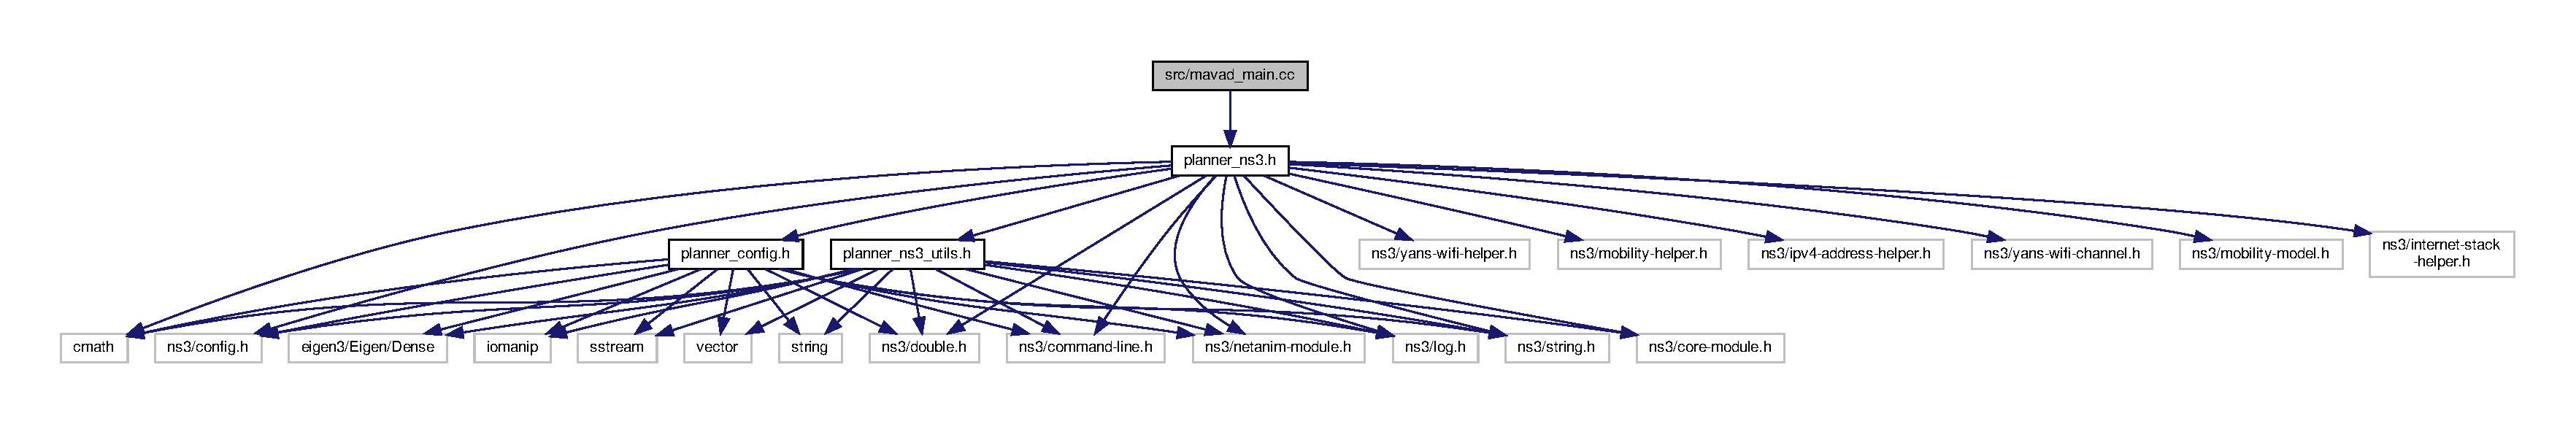
\includegraphics[width=350pt]{mavad__main_8cc__incl}
\end{center}
\end{figure}
\subsection*{Functions}
\begin{DoxyCompactItemize}
\item 
int \hyperlink{mavad__main_8cc_a3c04138a5bfe5d72780bb7e82a18e627}{main} (int argc, char $\ast$$\ast$argv)
\end{DoxyCompactItemize}


\subsection{Detailed Description}
Exucatable file for simulation, contains the main function. 

\begin{DoxyAuthor}{Author}
Ojit Mehta (\href{mailto:f20170372@goa.bits-pilani.ac.in}{\tt f20170372@goa.\+bits-\/pilani.\+ac.\+in}) 
\end{DoxyAuthor}
\begin{DoxyVersion}{Version}
0.\+1 
\end{DoxyVersion}
\begin{DoxyDate}{Date}
2021-\/03-\/29
\end{DoxyDate}
\begin{DoxyCopyright}{Copyright}
Copyright (c) 2021 
\end{DoxyCopyright}


\subsection{Function Documentation}
\mbox{\Hypertarget{mavad__main_8cc_a3c04138a5bfe5d72780bb7e82a18e627}\label{mavad__main_8cc_a3c04138a5bfe5d72780bb7e82a18e627}} 
\index{mavad\+\_\+main.\+cc@{mavad\+\_\+main.\+cc}!main@{main}}
\index{main@{main}!mavad\+\_\+main.\+cc@{mavad\+\_\+main.\+cc}}
\subsubsection{\texorpdfstring{main()}{main()}}
{\footnotesize\ttfamily int main (\begin{DoxyParamCaption}\item[{int}]{argc,  }\item[{char $\ast$$\ast$}]{argv }\end{DoxyParamCaption})}

Create an object of properties, give in phy\+Mode, rssi value and number of nodes

$<$ Initializing wihtout realtime simulation and with checksum disabled

$<$Set wifi without debug and disable pcap

$<$ Set IP

Create and start a Planner
%--- End generated contents ---

% Index
\backmatter
\newpage
\phantomsection
\clearemptydoublepage
\addcontentsline{toc}{chapter}{Index}
\printindex

\end{document}
